% Generated by Sphinx.
\documentclass[letterpaper,10pt,english]{manual}
\usepackage[utf8]{inputenc}
\usepackage[T1]{fontenc}
\usepackage{babel}
\usepackage{times}
\usepackage[Bjarne]{fncychap}
\usepackage{longtable}
\usepackage{sphinx}


\title{PyQGIS Documentation}
\date{December 06, 2010}
\release{1.4}
\author{Martin Dobias}
\newcommand{\sphinxlogo}{}
\renewcommand{\releasename}{Release}
\makeindex
\makemodindex

\makeatletter
\def\PYG@reset{\let\PYG@it=\relax \let\PYG@bf=\relax%
    \let\PYG@ul=\relax \let\PYG@tc=\relax%
    \let\PYG@bc=\relax \let\PYG@ff=\relax}
\def\PYG@tok#1{\csname PYG@tok@#1\endcsname}
\def\PYG@toks#1+{\ifx\relax#1\empty\else%
    \PYG@tok{#1}\expandafter\PYG@toks\fi}
\def\PYG@do#1{\PYG@bc{\PYG@tc{\PYG@ul{%
    \PYG@it{\PYG@bf{\PYG@ff{#1}}}}}}}
\def\PYG#1#2{\PYG@reset\PYG@toks#1+\relax+\PYG@do{#2}}

\def\PYG@tok@gd{\def\PYG@tc##1{\textcolor[rgb]{0.63,0.00,0.00}{##1}}}
\def\PYG@tok@gu{\let\PYG@bf=\textbf\def\PYG@tc##1{\textcolor[rgb]{0.50,0.00,0.50}{##1}}}
\def\PYG@tok@gt{\def\PYG@tc##1{\textcolor[rgb]{0.00,0.25,0.82}{##1}}}
\def\PYG@tok@gs{\let\PYG@bf=\textbf}
\def\PYG@tok@gr{\def\PYG@tc##1{\textcolor[rgb]{1.00,0.00,0.00}{##1}}}
\def\PYG@tok@cm{\let\PYG@it=\textit\def\PYG@tc##1{\textcolor[rgb]{0.25,0.50,0.56}{##1}}}
\def\PYG@tok@vg{\def\PYG@tc##1{\textcolor[rgb]{0.73,0.38,0.84}{##1}}}
\def\PYG@tok@m{\def\PYG@tc##1{\textcolor[rgb]{0.13,0.50,0.31}{##1}}}
\def\PYG@tok@mh{\def\PYG@tc##1{\textcolor[rgb]{0.13,0.50,0.31}{##1}}}
\def\PYG@tok@cs{\def\PYG@tc##1{\textcolor[rgb]{0.25,0.50,0.56}{##1}}\def\PYG@bc##1{\colorbox[rgb]{1.00,0.94,0.94}{##1}}}
\def\PYG@tok@ge{\let\PYG@it=\textit}
\def\PYG@tok@vc{\def\PYG@tc##1{\textcolor[rgb]{0.73,0.38,0.84}{##1}}}
\def\PYG@tok@il{\def\PYG@tc##1{\textcolor[rgb]{0.13,0.50,0.31}{##1}}}
\def\PYG@tok@go{\def\PYG@tc##1{\textcolor[rgb]{0.19,0.19,0.19}{##1}}}
\def\PYG@tok@cp{\def\PYG@tc##1{\textcolor[rgb]{0.00,0.44,0.13}{##1}}}
\def\PYG@tok@gi{\def\PYG@tc##1{\textcolor[rgb]{0.00,0.63,0.00}{##1}}}
\def\PYG@tok@gh{\let\PYG@bf=\textbf\def\PYG@tc##1{\textcolor[rgb]{0.00,0.00,0.50}{##1}}}
\def\PYG@tok@ni{\let\PYG@bf=\textbf\def\PYG@tc##1{\textcolor[rgb]{0.84,0.33,0.22}{##1}}}
\def\PYG@tok@nl{\let\PYG@bf=\textbf\def\PYG@tc##1{\textcolor[rgb]{0.00,0.13,0.44}{##1}}}
\def\PYG@tok@nn{\let\PYG@bf=\textbf\def\PYG@tc##1{\textcolor[rgb]{0.05,0.52,0.71}{##1}}}
\def\PYG@tok@no{\def\PYG@tc##1{\textcolor[rgb]{0.38,0.68,0.84}{##1}}}
\def\PYG@tok@na{\def\PYG@tc##1{\textcolor[rgb]{0.25,0.44,0.63}{##1}}}
\def\PYG@tok@nb{\def\PYG@tc##1{\textcolor[rgb]{0.00,0.44,0.13}{##1}}}
\def\PYG@tok@nc{\let\PYG@bf=\textbf\def\PYG@tc##1{\textcolor[rgb]{0.05,0.52,0.71}{##1}}}
\def\PYG@tok@nd{\let\PYG@bf=\textbf\def\PYG@tc##1{\textcolor[rgb]{0.33,0.33,0.33}{##1}}}
\def\PYG@tok@ne{\def\PYG@tc##1{\textcolor[rgb]{0.00,0.44,0.13}{##1}}}
\def\PYG@tok@nf{\def\PYG@tc##1{\textcolor[rgb]{0.02,0.16,0.49}{##1}}}
\def\PYG@tok@si{\let\PYG@it=\textit\def\PYG@tc##1{\textcolor[rgb]{0.44,0.63,0.82}{##1}}}
\def\PYG@tok@s2{\def\PYG@tc##1{\textcolor[rgb]{0.25,0.44,0.63}{##1}}}
\def\PYG@tok@vi{\def\PYG@tc##1{\textcolor[rgb]{0.73,0.38,0.84}{##1}}}
\def\PYG@tok@nt{\let\PYG@bf=\textbf\def\PYG@tc##1{\textcolor[rgb]{0.02,0.16,0.45}{##1}}}
\def\PYG@tok@nv{\def\PYG@tc##1{\textcolor[rgb]{0.73,0.38,0.84}{##1}}}
\def\PYG@tok@s1{\def\PYG@tc##1{\textcolor[rgb]{0.25,0.44,0.63}{##1}}}
\def\PYG@tok@gp{\let\PYG@bf=\textbf\def\PYG@tc##1{\textcolor[rgb]{0.78,0.36,0.04}{##1}}}
\def\PYG@tok@sh{\def\PYG@tc##1{\textcolor[rgb]{0.25,0.44,0.63}{##1}}}
\def\PYG@tok@ow{\let\PYG@bf=\textbf\def\PYG@tc##1{\textcolor[rgb]{0.00,0.44,0.13}{##1}}}
\def\PYG@tok@sx{\def\PYG@tc##1{\textcolor[rgb]{0.78,0.36,0.04}{##1}}}
\def\PYG@tok@bp{\def\PYG@tc##1{\textcolor[rgb]{0.00,0.44,0.13}{##1}}}
\def\PYG@tok@c1{\let\PYG@it=\textit\def\PYG@tc##1{\textcolor[rgb]{0.25,0.50,0.56}{##1}}}
\def\PYG@tok@kc{\let\PYG@bf=\textbf\def\PYG@tc##1{\textcolor[rgb]{0.00,0.44,0.13}{##1}}}
\def\PYG@tok@c{\let\PYG@it=\textit\def\PYG@tc##1{\textcolor[rgb]{0.25,0.50,0.56}{##1}}}
\def\PYG@tok@mf{\def\PYG@tc##1{\textcolor[rgb]{0.13,0.50,0.31}{##1}}}
\def\PYG@tok@err{\def\PYG@bc##1{\fcolorbox[rgb]{1.00,0.00,0.00}{1,1,1}{##1}}}
\def\PYG@tok@kd{\let\PYG@bf=\textbf\def\PYG@tc##1{\textcolor[rgb]{0.00,0.44,0.13}{##1}}}
\def\PYG@tok@ss{\def\PYG@tc##1{\textcolor[rgb]{0.32,0.47,0.09}{##1}}}
\def\PYG@tok@sr{\def\PYG@tc##1{\textcolor[rgb]{0.14,0.33,0.53}{##1}}}
\def\PYG@tok@mo{\def\PYG@tc##1{\textcolor[rgb]{0.13,0.50,0.31}{##1}}}
\def\PYG@tok@mi{\def\PYG@tc##1{\textcolor[rgb]{0.13,0.50,0.31}{##1}}}
\def\PYG@tok@kn{\let\PYG@bf=\textbf\def\PYG@tc##1{\textcolor[rgb]{0.00,0.44,0.13}{##1}}}
\def\PYG@tok@o{\def\PYG@tc##1{\textcolor[rgb]{0.40,0.40,0.40}{##1}}}
\def\PYG@tok@kr{\let\PYG@bf=\textbf\def\PYG@tc##1{\textcolor[rgb]{0.00,0.44,0.13}{##1}}}
\def\PYG@tok@s{\def\PYG@tc##1{\textcolor[rgb]{0.25,0.44,0.63}{##1}}}
\def\PYG@tok@kp{\def\PYG@tc##1{\textcolor[rgb]{0.00,0.44,0.13}{##1}}}
\def\PYG@tok@w{\def\PYG@tc##1{\textcolor[rgb]{0.73,0.73,0.73}{##1}}}
\def\PYG@tok@kt{\def\PYG@tc##1{\textcolor[rgb]{0.56,0.13,0.00}{##1}}}
\def\PYG@tok@sc{\def\PYG@tc##1{\textcolor[rgb]{0.25,0.44,0.63}{##1}}}
\def\PYG@tok@sb{\def\PYG@tc##1{\textcolor[rgb]{0.25,0.44,0.63}{##1}}}
\def\PYG@tok@k{\let\PYG@bf=\textbf\def\PYG@tc##1{\textcolor[rgb]{0.00,0.44,0.13}{##1}}}
\def\PYG@tok@se{\let\PYG@bf=\textbf\def\PYG@tc##1{\textcolor[rgb]{0.25,0.44,0.63}{##1}}}
\def\PYG@tok@sd{\let\PYG@it=\textit\def\PYG@tc##1{\textcolor[rgb]{0.25,0.44,0.63}{##1}}}

\def\PYGZbs{\char`\\}
\def\PYGZus{\char`\_}
\def\PYGZob{\char`\{}
\def\PYGZcb{\char`\}}
\def\PYGZca{\char`\^}
% for compatibility with earlier versions
\def\PYGZat{@}
\def\PYGZlb{[}
\def\PYGZrb{]}
\makeatother

\begin{document}

\maketitle
\tableofcontents
\hypertarget{--doc-index}{}


Contents:

\resetcurrentobjects
\hypertarget{--doc-intro}{}

\hypertarget{introduction}{}\chapter{Introduction}

This document is intended to work both as a tutorial and a reference guide. While it does not list all possible use cases, it should give
a good overview of the principal functionality.

Starting from 0.9 release, QGIS has optional scripting support using Python language. We've decided for Python as it's one of the most favourite
languages for scripting. PyQGIS bindings depend on SIP and PyQt4. The reason for using SIP instead of more widely used SWIG is that the whole
QGIS code depends on Qt libraries. Python bindings for Qt (PyQt) are done also using SIP and this allows seamless integration of PyQGIS with PyQt.
\begin{description}
\item[\textbf{TODO:}] \leavevmode
Getting PyQGIS to work (Manual compilation, Troubleshooting)

\end{description}

There are several ways how to use QGIS python bindings, they are covered in detail in the following sections:
\begin{itemize}
\item {} 
issue commands in Python console within QGIS

\item {} 
create and use plugins in Python

\item {} 
create custom applications based on QGIS API

\end{itemize}

There is a \href{http://doc.qgis.org/}{complete QGIS API} reference that documents the classes from the QGIS libraries.
Pythonic QGIS API is nearly identical to the API in C++.

There are some resources about programming with PyQGIS on \href{http://blog.qgis.org/}{QGIS blog}.
See \href{http://blog.qgis.org/?q=node/59}{QGIS tutorial ported to Python} for some examples of simple 3rd party apps.
A good resource when dealing with plugins is to download some plugins from \href{http://pyqgis.org/}{plugin repository} and examine their code.


\section{Python Console}

For scripting, it is possible to take advantage of integrated Python console. It can be opened from menu: \emph{Plugins \(\rightarrow\) Python Console}.
The console opens as a non-modal utility window:

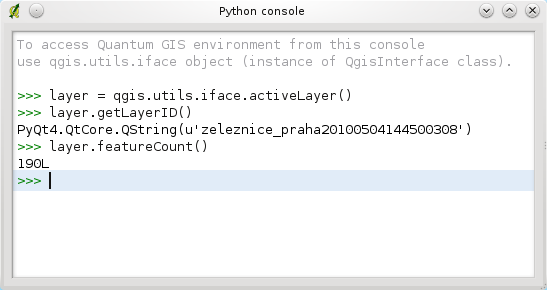
\includegraphics{console.png}

The screenshot above illustrates how to get the layer currntly selected in the layer list, show its ID and optionally, if it is a vector layer, show the feature count.
For interaction with QGIS environment, there is \code{qgis.utils.iface} variable, which is instance of \code{QgisInterface}. This interface allows access to the map
canvas, menus, toolbars and other parts of the QGIS application.

For convenience of the user, the following statements are executed when the console is started (in future it will be possible to set further initial commands):

\begin{Verbatim}[commandchars=\\\{\}]
\PYG{k+kn}{from} \PYG{n+nn}{qgis.core} \PYG{k+kn}{import} \PYG{o}{*}
\PYG{k+kn}{import} \PYG{n+nn}{qgis.utils}
\end{Verbatim}

For those which use the console often, it may be useful to set a shortcut for triggering the console (within menu \emph{Settings \(\rightarrow\) Configure shortcuts...})


\section{Python Plugins}

Quantum GIS allows enhancement of its functionality using plugins. This was originally possible only with C++ language. With the addition of Python support to QGIS,
it is also possible to use plugins written in Python. Great advantages over C++ plugins is the simplicity of distribution (no compiling for each platform needed)
and easier development.

Many plugins covering various functionality have been written since the introduction of Python support. Plugin installer allows users to easily fetch, upgrade and
remove Python plugins. See \href{http://www.qgis.org/wiki/Python\_Plugin\_Repositories}{Python Plugin Repositories} page for various sources of plugins.

Creating plugins in Python is simple, see \hyperlink{plugins}{\emph{Developing Python Plugins}} for detailed instructions.


\section{Python Applications}

Often when processing some GIS data, it is handy to create some scripts for automating the process instead of doing the same task again and again.
With PyQGIS, this is perfectly possible --- import the \code{qgis.core} module, initialize it and you are ready for the processing.

Or you may want to create an interactive application that uses some GIS functionality --- measure some data, export a map in PDF or any other functionality.
The \code{qgis.gui} module additionally brings various GUI components, most notably the map canvas widget that can be very easily incorporated into the
application with support for zooming, panning and/or any further custom map tools.


\subsection{Using PyQGIS in custom application}

Note: do \emph{not} use \code{qgis.py} as a name for your test script --- python will not be able to import the bindings as the script's name will shadow them.

First of all you have to import qgis module, set QGIS path where to search for resources - database of projections, providers etc.
When you set prefix path with second argument set as \code{True}, QGIS will initialize all paths with standard dir under the prefix directory.
Calling \code{initQgis()} function is important to let QGIS search for the available providers.

\begin{Verbatim}[commandchars=\\\{\}]
\PYG{k+kn}{from} \PYG{n+nn}{qgis.core} \PYG{k+kn}{import} \PYG{o}{*}

\PYG{c}{\# supply path to where is your qgis installed}
\PYG{n}{QgsApplication}\PYG{o}{.}\PYG{n}{setPrefixPath}\PYG{p}{(}\PYG{l+s}{"}\PYG{l+s}{/path/to/qgis/installation}\PYG{l+s}{"}\PYG{p}{,} \PYG{n+nb+bp}{True}\PYG{p}{)}

\PYG{c}{\# load providers}
\PYG{n}{QgsApplication}\PYG{o}{.}\PYG{n}{initQgis}\PYG{p}{(}\PYG{p}{)}
\end{Verbatim}

Now you can work with QGIS API - load layers and do some processing or fire up a GUI with a map canvas. The possibilities are endless :-)

When you are done with using QGIS library, call \code{exitQgis()} to make sure that everything is cleaned up (e.g. clear map layer registry and delete layers):

\begin{Verbatim}[commandchars=\\\{\}]
\PYG{n}{QgsApplication}\PYG{o}{.}\PYG{n}{exitQgis}\PYG{p}{(}\PYG{p}{)}
\end{Verbatim}


\subsection{Running Custom Applications}

You will need to tell your system where to search for QGIS libraries and appropriate Python modules if they are not in a well-known location --- otherwise Python
will complain:

\begin{Verbatim}[commandchars=\\\{\}]
\PYG{g+gp}{\textgreater{}\textgreater{}\textgreater{} }\PYG{k+kn}{import} \PYG{n+nn}{qgis.core}
\PYG{g+go}{ImportError: No module named qgis.core}
\end{Verbatim}

This can be fixed by setting the \code{PYTHONPATH} environment variable. In the following commands, \code{qgispath} should be replaced with your actual QGIS installation path:
\begin{itemize}
\item {} 
on Linux: \textbf{export PYTHONPATH=/qgispath/share/qgis/python}

\item {} 
on Windows: \textbf{set PYTHONPATH=c:\textbackslash{}qgispath\textbackslash{}python}

\end{itemize}

The path to the PyQGIS modules is now known, however they depend on \code{qgis\_core} and \code{qgis\_gui} libraries (the Python modules serve only as wrappers). Path to these
libraries is typically unknown for the operating system, so you get an import error again (the message might vary depending on the system):

\begin{Verbatim}[commandchars=\\\{\}]
\PYG{g+gp}{\textgreater{}\textgreater{}\textgreater{} }\PYG{k+kn}{import} \PYG{n+nn}{qgis.core}
\PYG{g+go}{ImportError: libqgis\PYGZus{}core.so.1.5.0: cannot open shared object file: No such file or directory}
\end{Verbatim}

Fix this by adding the directories where the QGIS libraries reside to search path of the dynamic linker:
\begin{itemize}
\item {} 
on Linux: \textbf{export LD\_LIBRARY\_PATH=/qgispath/lib}

\item {} 
on Windows: \textbf{set PATH=C:\textbackslash{}qgispath;\%PATH\%}

\end{itemize}

These commands can be put into a bootstrap script that will take care of the startup.
When deploying custom applications using PyQGIS, there are usually two possibilities:
\begin{itemize}
\item {} 
require user to install QGIS on his platform prior to installing your application. The application installer should look for default locations of QGIS libraries
and allow user to set the path if not found. This approach has the advantage of being simpler, however it requires user to do more steps.

\item {} 
package QGIS together with your application. Releasing the application may be more challenging and the package will be larger, but the user will be saved from the
burden of downloading and installing additional pieces of software.

\end{itemize}

The two deployment models can be mixed - deploy standalone application on Windows and Mac OS X, for Linux leave the installation of QGIS up to user and his package manager.

\resetcurrentobjects
\hypertarget{--doc-loadlayer}{}

\chapter{Loading Layers}

Let's open some layers with data. QGIS recognizes vector and raster layers. Additionally, custom layer types are available, but we are not going to discuss them here.


\section{Vector Layers}

To load a vector layer, specify layer's data source identifier, name for the layer and provider's name:

\begin{Verbatim}[commandchars=\\\{\}]
\PYG{n}{layer} \PYG{o}{=} \PYG{n}{QgsVectorLayer}\PYG{p}{(}\PYG{n}{data\PYGZus{}source}\PYG{p}{,} \PYG{n}{layer\PYGZus{}name}\PYG{p}{,} \PYG{n}{provider\PYGZus{}name}\PYG{p}{)}
\PYG{k}{if} \PYG{o+ow}{not} \PYG{n}{layer}\PYG{o}{.}\PYG{n}{isValid}\PYG{p}{(}\PYG{p}{)}\PYG{p}{:}
  \PYG{k}{print} \PYG{l+s}{"}\PYG{l+s}{Layer failed to load!}\PYG{l+s}{"}
\end{Verbatim}

The data source identifier is a string and it is specific to each vector data provider. Layer's name is used in the layer list widget.
It is important to check whether the layer has been loaded successfully. If it was not, an invalid layer instance is returned.

The following list shows how to access various data sources using vector data providers:
\begin{itemize}
\item {} 
OGR library (shapefiles and many other file formats) - data source is the path to the file:

\begin{Verbatim}[commandchars=\\\{\}]
\PYG{n}{vlayer} \PYG{o}{=} \PYG{n}{QgsVectorLayer}\PYG{p}{(}\PYG{l+s}{"}\PYG{l+s}{/path/to/shapefile/file.shp}\PYG{l+s}{"}\PYG{p}{,} \PYG{l+s}{"}\PYG{l+s}{layer\PYGZus{}name\PYGZus{}you\PYGZus{}like}\PYG{l+s}{"}\PYG{p}{,} \PYG{l+s}{"}\PYG{l+s}{ogr}\PYG{l+s}{"}\PYG{p}{)}
\end{Verbatim}

\item {} 
PostGIS database - data source is a string with all information needed to create a connection to PostgreSQL database. \code{QgsDataSourceURI} class can generate this string for you.
Note that QGIS has to be compiled with Postgres support, otherwise this provider isn't available.

\begin{Verbatim}[commandchars=\\\{\}]
\PYG{n}{uri} \PYG{o}{=} \PYG{n}{QgsDataSourceURI}\PYG{p}{(}\PYG{p}{)}
\PYG{c}{\# set host name, port, database name, username and password}
\PYG{n}{uri}\PYG{o}{.}\PYG{n}{setConnection}\PYG{p}{(}\PYG{l+s}{"}\PYG{l+s}{localhost}\PYG{l+s}{"}\PYG{p}{,} \PYG{l+s}{"}\PYG{l+s}{5432}\PYG{l+s}{"}\PYG{p}{,} \PYG{l+s}{"}\PYG{l+s}{dbname}\PYG{l+s}{"}\PYG{p}{,} \PYG{l+s}{"}\PYG{l+s}{johny}\PYG{l+s}{"}\PYG{p}{,} \PYG{l+s}{"}\PYG{l+s}{xxx}\PYG{l+s}{"}\PYG{p}{)}
\PYG{c}{\# set database schema, table name, geometry column and optionaly subset (WHERE clause)}
\PYG{n}{uri}\PYG{o}{.}\PYG{n}{setDataSource}\PYG{p}{(}\PYG{l+s}{"}\PYG{l+s}{public}\PYG{l+s}{"}\PYG{p}{,} \PYG{l+s}{"}\PYG{l+s}{roads}\PYG{l+s}{"}\PYG{p}{,} \PYG{l+s}{"}\PYG{l+s}{the\PYGZus{}geom}\PYG{l+s}{"}\PYG{p}{,} \PYG{l+s}{"}\PYG{l+s}{cityid = 2643}\PYG{l+s}{"}\PYG{p}{)}

\PYG{n}{vlayer} \PYG{o}{=} \PYG{n}{QgsVectorLayer}\PYG{p}{(}\PYG{n}{uri}\PYG{o}{.}\PYG{n}{uri}\PYG{p}{(}\PYG{p}{)}\PYG{p}{,} \PYG{l+s}{"}\PYG{l+s}{layer\PYGZus{}name\PYGZus{}you\PYGZus{}like}\PYG{l+s}{"}\PYG{p}{,} \PYG{l+s}{"}\PYG{l+s}{postgres}\PYG{l+s}{"}\PYG{p}{)}
\end{Verbatim}

\item {} 
CSV or other delimited text files - to open a file with a semicolon as a delimiter, with field ``x'' for x-coordinate and field ``y'' with y-coordinate you would use something like this:

\begin{Verbatim}[commandchars=\\\{\}]
\PYG{n}{uri} \PYG{o}{=} \PYG{l+s}{"}\PYG{l+s}{/some/path/file.csv?delimiter=}\PYG{l+s+si}{\%s}\PYG{l+s}{\&xField=}\PYG{l+s+si}{\%s}\PYG{l+s}{\&yField=}\PYG{l+s+si}{\%s}\PYG{l+s}{"} \PYG{o}{\%} \PYG{p}{(}\PYG{l+s}{"}\PYG{l+s}{;}\PYG{l+s}{"}\PYG{p}{,} \PYG{l+s}{"}\PYG{l+s}{x}\PYG{l+s}{"}\PYG{p}{,} \PYG{l+s}{"}\PYG{l+s}{y}\PYG{l+s}{"}\PYG{p}{)}
\PYG{n}{vlayer} \PYG{o}{=} \PYG{n}{QgsVectorLayer}\PYG{p}{(}\PYG{n}{uri}\PYG{p}{,} \PYG{l+s}{"}\PYG{l+s}{layer\PYGZus{}name\PYGZus{}you\PYGZus{}like}\PYG{l+s}{"}\PYG{p}{,} \PYG{l+s}{"}\PYG{l+s}{delimitedtext}\PYG{l+s}{"}\PYG{p}{)}
\end{Verbatim}

\item {} 
GPX files - the ``gpx'' data provider reads tracks, routes and waypoints from gpx files. To open a file, the type (track/route/waypoint) needs to be specified as part of the url:

\begin{Verbatim}[commandchars=\\\{\}]
\PYG{n}{uri} \PYG{o}{=} \PYG{l+s}{"}\PYG{l+s}{path/to/gpx/file.gpx?type=track}\PYG{l+s}{"}
\PYG{n}{vlayer} \PYG{o}{=} \PYG{n}{QgsVectorLayer}\PYG{p}{(}\PYG{n}{uri}\PYG{p}{,} \PYG{l+s}{"}\PYG{l+s}{layer\PYGZus{}name\PYGZus{}you\PYGZus{}like}\PYG{l+s}{"}\PYG{p}{,} \PYG{l+s}{"}\PYG{l+s}{gpx}\PYG{l+s}{"}\PYG{p}{)}
\end{Verbatim}

\item {} 
SpatiaLite database - supported from QGIS v1.1. Similarly to PostGIS databases, \code{QgsDataSourceURI} can be used for generation of data source identifier:

\begin{Verbatim}[commandchars=\\\{\}]
\PYG{n}{uri} \PYG{o}{=} \PYG{n}{QgsDataSourceURI}\PYG{p}{(}\PYG{p}{)}
\PYG{n}{uri}\PYG{o}{.}\PYG{n}{setDatabase}\PYG{p}{(}\PYG{l+s}{'}\PYG{l+s}{/home/martin/test-2.3.sqlite}\PYG{l+s}{'}\PYG{p}{)}
\PYG{n}{uri}\PYG{o}{.}\PYG{n}{setDataSource}\PYG{p}{(}\PYG{l+s}{'}\PYG{l+s}{'}\PYG{p}{,}\PYG{l+s}{'}\PYG{l+s}{Towns}\PYG{l+s}{'}\PYG{p}{,} \PYG{l+s}{'}\PYG{l+s}{Geometry}\PYG{l+s}{'}\PYG{p}{)}

\PYG{n}{vlayer} \PYG{o}{=} \PYG{n}{QgsVectorLayer}\PYG{p}{(}\PYG{n}{uri}\PYG{o}{.}\PYG{n}{uri}\PYG{p}{(}\PYG{p}{)}\PYG{p}{,} \PYG{l+s}{'}\PYG{l+s}{Towns}\PYG{l+s}{'}\PYG{p}{,} \PYG{l+s}{'}\PYG{l+s}{spatialite}\PYG{l+s}{'}\PYG{p}{)}
\end{Verbatim}

\end{itemize}


\section{Raster Layers}

For accessing raster files, GDAL library is used. It supports a wide range of file formats. In case you have troubles with opening some files, check whether
your GDAL has support for the particular format (not all formats are available by default). To load a raster from a file, specify its file name and base name:

\begin{Verbatim}[commandchars=\\\{\}]
\PYG{n}{fileName} \PYG{o}{=} \PYG{l+s}{"}\PYG{l+s}{/path/to/raster/file.tif}\PYG{l+s}{"}
\PYG{n}{fileInfo} \PYG{o}{=} \PYG{n}{QFileInfo}\PYG{p}{(}\PYG{n}{fileName}\PYG{p}{)}
\PYG{n}{baseName} \PYG{o}{=} \PYG{n}{fileInfo}\PYG{o}{.}\PYG{n}{baseName}\PYG{p}{(}\PYG{p}{)}
\PYG{n}{rlayer} \PYG{o}{=} \PYG{n}{QgsRasterLayer}\PYG{p}{(}\PYG{n}{fileName}\PYG{p}{,} \PYG{n}{baseName}\PYG{p}{)}
\PYG{k}{if} \PYG{o+ow}{not} \PYG{n}{rlayer}\PYG{o}{.}\PYG{n}{isValid}\PYG{p}{(}\PYG{p}{)}\PYG{p}{:}
  \PYG{k}{print} \PYG{l+s}{"}\PYG{l+s}{Layer failed to load!}\PYG{l+s}{"}
\end{Verbatim}

Alternatively you can load a raster layer from WMS server. However currently it's not possible to access GetCapabilities response from API - you have to know what layers you want:

\begin{Verbatim}[commandchars=\\\{\}]
\PYG{n}{url} \PYG{o}{=} \PYG{l+s}{'}\PYG{l+s}{http://wms.jpl.nasa.gov/wms.cgi}\PYG{l+s}{'}
\PYG{n}{layers} \PYG{o}{=} \PYG{p}{[} \PYG{l+s}{'}\PYG{l+s}{global\PYGZus{}mosaic}\PYG{l+s}{'} \PYG{p}{]}
\PYG{n}{styles} \PYG{o}{=} \PYG{p}{[} \PYG{l+s}{'}\PYG{l+s}{pseudo}\PYG{l+s}{'} \PYG{p}{]}
\PYG{n}{format} \PYG{o}{=} \PYG{l+s}{'}\PYG{l+s}{image/jpeg}\PYG{l+s}{'}
\PYG{n}{crs} \PYG{o}{=} \PYG{l+s}{'}\PYG{l+s}{EPSG:4326}\PYG{l+s}{'}
\PYG{n}{rlayer} \PYG{o}{=} \PYG{n}{QgsRasterLayer}\PYG{p}{(}\PYG{l+m+mi}{0}\PYG{p}{,} \PYG{n}{url}\PYG{p}{,} \PYG{l+s}{'}\PYG{l+s}{some layer name}\PYG{l+s}{'}\PYG{p}{,} \PYG{l+s}{'}\PYG{l+s}{wms}\PYG{l+s}{'}\PYG{p}{,} \PYG{n}{layers}\PYG{p}{,} \PYG{n}{styles}\PYG{p}{,} \PYG{n}{format}\PYG{p}{,} \PYG{n}{crs}\PYG{p}{)}
\PYG{k}{if} \PYG{o+ow}{not} \PYG{n}{rlayer}\PYG{o}{.}\PYG{n}{isValid}\PYG{p}{(}\PYG{p}{)}\PYG{p}{:}
  \PYG{k}{print} \PYG{l+s}{"}\PYG{l+s}{Layer failed to load!}\PYG{l+s}{"}
\end{Verbatim}


\section{Map Layer Registry}

If you would like to use the opened layers for rendering, do not forget to add them to map layer registry. The map layer registry takes ownership of layers
and they can be later accessed from any part of the application by their unique ID. When the layer is removed from map layer registry, it gets deleted, too.

Adding a layer to the registry:

\begin{Verbatim}[commandchars=\\\{\}]
\PYG{n}{QgsMapLayerRegistry}\PYG{o}{.}\PYG{n}{instance}\PYG{p}{(}\PYG{p}{)}\PYG{o}{.}\PYG{n}{addMapLayer}\PYG{p}{(}\PYG{n}{layer}\PYG{p}{)}
\end{Verbatim}

Layers are destroyed automatically on exit, however if you want to delete the layer explicitly, use:

\begin{Verbatim}[commandchars=\\\{\}]
\PYG{n}{QgsMapLayerRegistry}\PYG{o}{.}\PYG{n}{instance}\PYG{p}{(}\PYG{p}{)}\PYG{o}{.}\PYG{n}{removeMapLayer}\PYG{p}{(}\PYG{n}{layer\PYGZus{}id}\PYG{p}{)}
\end{Verbatim}
\begin{description}
\item[\textbf{TODO:}] \leavevmode
More about map layer registry?

\end{description}

\resetcurrentobjects
\hypertarget{--doc-raster}{}

\hypertarget{raster}{}\chapter{Using Raster Layers}

This sections lists various operations you can do with raster layers.


\section{Layer Details}

A raster layer consists of one or more raster bands - it is referred to as either single band or multi band raster.
One band represents a matrix of values. Usual color image (e.g. aerial photo) is a raster consisting of red, blue and green band.
Single band layers typically represent either continuous variables (e.g. elevation) or discrete variables (e.g. land use).
In some cases, a raster layer comes with a palette and raster values refer to colors stored in the palette.

\begin{Verbatim}[commandchars=\\\{\}]
\PYG{g+gp}{\textgreater{}\textgreater{}\textgreater{} }\PYG{n}{rlayer}\PYG{o}{.}\PYG{n}{width}\PYG{p}{(}\PYG{p}{)}\PYG{p}{,} \PYG{n}{rlayer}\PYG{o}{.}\PYG{n}{height}\PYG{p}{(}\PYG{p}{)}
\PYG{g+go}{(812, 301)}
\PYG{g+gp}{\textgreater{}\textgreater{}\textgreater{} }\PYG{n}{rlayer}\PYG{o}{.}\PYG{n}{extent}\PYG{p}{(}\PYG{p}{)}\PYG{o}{.}\PYG{n}{toString}\PYG{p}{(}\PYG{p}{)}
\PYG{g+go}{PyQt4.QtCore.QString(u'12.095833,48.552777 : 18.863888,51.056944')}
\PYG{g+gp}{\textgreater{}\textgreater{}\textgreater{} }\PYG{n}{rlayer}\PYG{o}{.}\PYG{n}{rasterType}\PYG{p}{(}\PYG{p}{)}
\PYG{g+go}{2  \# 0 = GrayOrUndefined (single band), 1 = Palette (single band), 2 = Multiband}
\PYG{g+gp}{\textgreater{}\textgreater{}\textgreater{} }\PYG{n}{rlayer}\PYG{o}{.}\PYG{n}{bandCount}\PYG{p}{(}\PYG{p}{)}
\PYG{g+go}{3}
\PYG{g+gp}{\textgreater{}\textgreater{}\textgreater{} }\PYG{n}{rlayer}\PYG{o}{.}\PYG{n}{metadata}\PYG{p}{(}\PYG{p}{)}
\PYG{g+go}{PyQt4.QtCore.QString(u'\textless{}p class="glossy"\textgreater{}Driver:\textless{}/p\textgreater{}...')}
\PYG{g+gp}{\textgreater{}\textgreater{}\textgreater{} }\PYG{n}{rlayer}\PYG{o}{.}\PYG{n}{hasPyramids}\PYG{p}{(}\PYG{p}{)}
\PYG{g+go}{False}
\end{Verbatim}


\section{Drawing Style}

When a raster layer is loaded, it gets a default drawing style based on its type. It can be altered either in raster layer properties or programmatically.
The following drawing styles exist:

\begin{tabulary}{\textwidth}{|L|L|L|}
\hline
\textbf{
Index
} & \textbf{
Constant: QgsRasterLater.X
} & \textbf{
Comment
}\\
\hline

1
 & 
SingleBandGray
 & 
Single band image drawn as a range of gray colors
\\

2
 & 
SingleBandPseudoColor
 & 
Single band image drawn using a pseudocolor algorithm
\\

3
 & 
PalettedColor
 & 
``Palette'' image drawn using color table
\\

4
 & 
PalettedSingleBandGray
 & 
``Palette'' layer drawn in gray scale
\\

5
 & 
PalettedSingleBandPseudoColor
 & 
``Palette'' layerdrawn using a pseudocolor algorithm
\\

7
 & 
MultiBandSingleBandGray
 & 
Layer containing 2 or more bands, but a single band drawn as a range of gray colors
\\

8
 & 
MultiBandSingleBandPseudoColor
 & 
Layer containing 2 or more bands, but a single band drawn using a pseudocolor algorithm
\\

9
 & 
MultiBandColor
 & 
Layer containing 2 or more bands, mapped to RGB color space.
\\
\hline
\end{tabulary}


To query the current drawing style:

\begin{Verbatim}[commandchars=\\\{\}]
\PYG{g+gp}{\textgreater{}\textgreater{}\textgreater{} }\PYG{n}{rlayer}\PYG{o}{.}\PYG{n}{drawingStyle}\PYG{p}{(}\PYG{p}{)}
\PYG{g+go}{9}
\end{Verbatim}

Single band raster layers can be drawn either in gray colors (low values = black, high values = white) or with a pseudocolor algorithm
that assigns colors for values from the single band. Single band rasters with a palette can be additionally drawn using their palette.
Multiband layers are typically drawn by mapping the bands to RGB colors. Other possibility is to use just one band for gray or pseudocolor
drawing.

The following sections explain how to query and modify the layer drawing style. After doing the changes, you might want to force update
of map canvas, see \hyperlink{refresh-layer}{\emph{Refresing Layers}}.

\textbf{TODO:} contrast enhancements, transparency (no data), user defined min/max, band statistics


\section{Single Band Rasters}

They are rendered in gray colors by default. To change the drawing style to pseudocolor:

\begin{Verbatim}[commandchars=\\\{\}]
\PYG{g+gp}{\textgreater{}\textgreater{}\textgreater{} }\PYG{n}{rlayer}\PYG{o}{.}\PYG{n}{setDrawingStyle}\PYG{p}{(}\PYG{n}{QgsRasterLayer}\PYG{o}{.}\PYG{n}{SingleBandPseudoColor}\PYG{p}{)}
\PYG{g+gp}{\textgreater{}\textgreater{}\textgreater{} }\PYG{n}{rlayer}\PYG{o}{.}\PYG{n}{setColorShadingAlgorithm}\PYG{p}{(}\PYG{n}{QgsRasterLayer}\PYG{o}{.}\PYG{n}{PseudoColorShader}\PYG{p}{)}
\end{Verbatim}

The \code{PseudoColorShader} is a basic shader that highlighs low values in blue and high values in red. Another, \code{FreakOutShader} uses
more fancy colors and according to the documentation, it will frighten your granny and make your dogs howl.

There is also \code{ColorRampShader} which maps the colors as specified by its color map. It has three modes of interpolation of values:
\begin{itemize}
\item {} 
linear (\code{INTERPOLATED}): resulting color is linearly interpolated from the color map entries above and below the actual pixel value

\item {} 
discrete (\code{DISCRETE}): color is used from the color map entry with equal or higher value

\item {} 
exact (\code{EXACT}): color is not interpolated, only the pixels with value equal to color map entries are drawn

\end{itemize}

To set an interpolated color ramp shader ranging from green to yellow color (for pixel values from 0 to 255):

\begin{Verbatim}[commandchars=\\\{\}]
\PYG{g+gp}{\textgreater{}\textgreater{}\textgreater{} }\PYG{n}{rlayer}\PYG{o}{.}\PYG{n}{setColorShadingAlgorithm}\PYG{p}{(}\PYG{n}{QgsRasterLayer}\PYG{o}{.}\PYG{n}{ColorRampShader}\PYG{p}{)}
\PYG{g+gp}{\textgreater{}\textgreater{}\textgreater{} }\PYG{n}{lst} \PYG{o}{=} \PYG{p}{[} \PYG{n}{QgsColorRampShader}\PYG{o}{.}\PYG{n}{ColorRampItem}\PYG{p}{(}\PYG{l+m+mi}{0}\PYG{p}{,} \PYG{n}{QColor}\PYG{p}{(}\PYG{l+m+mi}{0}\PYG{p}{,}\PYG{l+m+mi}{255}\PYG{p}{,}\PYG{l+m+mi}{0}\PYG{p}{)}\PYG{p}{)}\PYG{p}{,} \PYG{n}{QgsColorRampShader}\PYG{o}{.}\PYG{n}{ColorRampItem}\PYG{p}{(}\PYG{l+m+mi}{255}\PYG{p}{,} \PYG{n}{QColor}\PYG{p}{(}\PYG{l+m+mi}{255}\PYG{p}{,}\PYG{l+m+mi}{255}\PYG{p}{,}\PYG{l+m+mi}{0}\PYG{p}{)}\PYG{p}{)} \PYG{p}{]}
\PYG{g+gp}{\textgreater{}\textgreater{}\textgreater{} }\PYG{n}{fcn} \PYG{o}{=} \PYG{n}{rlayer}\PYG{o}{.}\PYG{n}{rasterShader}\PYG{p}{(}\PYG{p}{)}\PYG{o}{.}\PYG{n}{rasterShaderFunction}\PYG{p}{(}\PYG{p}{)}
\PYG{g+gp}{\textgreater{}\textgreater{}\textgreater{} }\PYG{n}{fcn}\PYG{o}{.}\PYG{n}{setColorRampType}\PYG{p}{(}\PYG{n}{QgsColorRampShader}\PYG{o}{.}\PYG{n}{INTERPOLATED}\PYG{p}{)}
\PYG{g+gp}{\textgreater{}\textgreater{}\textgreater{} }\PYG{n}{fcn}\PYG{o}{.}\PYG{n}{setColorRampItemList}\PYG{p}{(}\PYG{n}{lst}\PYG{p}{)}
\end{Verbatim}

To return back to default gray levels, use:

\begin{Verbatim}[commandchars=\\\{\}]
\PYG{g+gp}{\textgreater{}\textgreater{}\textgreater{} }\PYG{n}{rlayer}\PYG{o}{.}\PYG{n}{setDrawingStyle}\PYG{p}{(}\PYG{n}{QgsRasterLayer}\PYG{o}{.}\PYG{n}{SingleBandGray}\PYG{p}{)}
\end{Verbatim}


\section{Multi Band Rasters}

By default, QGIS maps the first three bands to red, green and blue values to create a color image (this is the \code{MultiBandColor} drawing style.
In some cases you might want to override these setting. The following code interchanges red band (1) and green band (2):

\begin{Verbatim}[commandchars=\\\{\}]
\PYG{g+gp}{\textgreater{}\textgreater{}\textgreater{} }\PYG{n}{rlayer}\PYG{o}{.}\PYG{n}{setGreenBandName}\PYG{p}{(}\PYG{n}{rlayer}\PYG{o}{.}\PYG{n}{bandName}\PYG{p}{(}\PYG{l+m+mi}{1}\PYG{p}{)}\PYG{p}{)}
\PYG{g+gp}{\textgreater{}\textgreater{}\textgreater{} }\PYG{n}{rlayer}\PYG{o}{.}\PYG{n}{setRedBandName}\PYG{p}{(}\PYG{n}{rlayer}\PYG{o}{.}\PYG{n}{bandName}\PYG{p}{(}\PYG{l+m+mi}{2}\PYG{p}{)}\PYG{p}{)}
\end{Verbatim}

In case only one band is necessary for visualization of the raster, single band drawing can be chosen - either gray levels or pseudocolor,
see previous section:

\begin{Verbatim}[commandchars=\\\{\}]
\PYG{g+gp}{\textgreater{}\textgreater{}\textgreater{} }\PYG{n}{rlayer}\PYG{o}{.}\PYG{n}{setDrawingStyle}\PYG{p}{(}\PYG{n}{QgsRasterLayer}\PYG{o}{.}\PYG{n}{MultiBandSingleBandPseudoColor}\PYG{p}{)}
\PYG{g+gp}{\textgreater{}\textgreater{}\textgreater{} }\PYG{n}{rlayer}\PYG{o}{.}\PYG{n}{setGrayBandName}\PYG{p}{(}\PYG{n}{rlayer}\PYG{o}{.}\PYG{n}{bandName}\PYG{p}{(}\PYG{l+m+mi}{1}\PYG{p}{)}\PYG{p}{)}
\PYG{g+gp}{\textgreater{}\textgreater{}\textgreater{} }\PYG{n}{rlayer}\PYG{o}{.}\PYG{n}{setColorShadingAlgorithm}\PYG{p}{(}\PYG{n}{QgsRasterLayer}\PYG{o}{.}\PYG{n}{PseudoColorShader}\PYG{p}{)}
\PYG{g+gp}{\textgreater{}\textgreater{}\textgreater{} }\PYG{c}{\# now set the shader}
\end{Verbatim}
\hypertarget{refresh-layer}{}

\section{Refresing Layers}

If you do change layer symbology and would like ensure that the changes are immediately visible to the user, call these methods:

\begin{Verbatim}[commandchars=\\\{\}]
\PYG{k}{if} \PYG{n+nb}{hasattr}\PYG{p}{(}\PYG{n}{layer}\PYG{p}{,} \PYG{l+s}{"}\PYG{l+s}{setCacheImage}\PYG{l+s}{"}\PYG{p}{)}\PYG{p}{:} \PYG{n}{layer}\PYG{o}{.}\PYG{n}{setCacheImage}\PYG{p}{(}\PYG{n+nb+bp}{None}\PYG{p}{)}
\PYG{n}{layer}\PYG{o}{.}\PYG{n}{triggerRepaint}\PYG{p}{(}\PYG{p}{)}
\end{Verbatim}

The first call will ensure that the cached image of rendered layer is erased in case render caching is turned on. This functionality is available from QGIS 1.4,
in previous versions this function does not exist - to make sure that the code works with all versions of QGIS, we first check whether the method exists.

The second call emits signal that will force any map canvas containing the layer to issue a refresh.

In case you have changed layer symbology (see sections about raster and vector layers on how to do that), you might want to force QGIS to update the layer
symbology in the layer list (legend) widget. This can be done as follows (\code{iface} is an instance of QgisInterface):

\begin{Verbatim}[commandchars=\\\{\}]
\PYG{n}{iface}\PYG{o}{.}\PYG{n}{legendInterface}\PYG{p}{(}\PYG{p}{)}\PYG{o}{.}\PYG{n}{refreshLayerSymbology}\PYG{p}{(}\PYG{n}{layer}\PYG{p}{)}
\end{Verbatim}


\section{Query Values}

To do a query on value of bands of raster layer at some specified point:

\begin{Verbatim}[commandchars=\\\{\}]
\PYG{n}{ident} \PYG{o}{=} \PYG{n}{rlayer}\PYG{o}{.}\PYG{n}{identify}\PYG{p}{(}\PYG{n}{QgsPoint}\PYG{p}{(}\PYG{l+m+mf}{15.30}\PYG{p}{,}\PYG{l+m+mf}{40.98}\PYG{p}{)}\PYG{p}{)}
\PYG{k}{for} \PYG{p}{(}\PYG{n}{k}\PYG{p}{,}\PYG{n}{v}\PYG{p}{)} \PYG{o+ow}{in} \PYG{n}{ident}\PYG{o}{.}\PYG{n}{iteritems}\PYG{p}{(}\PYG{p}{)}\PYG{p}{:}
  \PYG{k}{print} \PYG{n+nb}{str}\PYG{p}{(}\PYG{n}{k}\PYG{p}{)}\PYG{p}{,}\PYG{l+s}{"}\PYG{l+s}{:}\PYG{l+s}{"}\PYG{p}{,}\PYG{n+nb}{str}\PYG{p}{(}\PYG{n}{v}\PYG{p}{)}
\end{Verbatim}

The identify function returns a dictionary - keys are band names, values are the values at chosen point.
Both key and value are QString instances so to see actual value you'll need to convert them to python strings (as shown in code snippet).

\resetcurrentobjects
\hypertarget{--doc-vector}{}

\hypertarget{vector}{}\chapter{Using Vector Layers}

This section summarizes various actions that can be done with vector layers.
\begin{description}
\item[\textbf{TODO:}] \leavevmode
Editing, Layer vs. Data provider, ...

\end{description}


\section{Iterating over Vector Layer}

Below is an example how to go through the features of the layer. To read features from layer, initialize the retieval with \code{select()} and then use \code{nextFeature()} calls:

\begin{Verbatim}[commandchars=\\\{\}]
\PYG{n}{provider} \PYG{o}{=} \PYG{n}{vlayer}\PYG{o}{.}\PYG{n}{dataProvider}\PYG{p}{(}\PYG{p}{)}

\PYG{n}{feat} \PYG{o}{=} \PYG{n}{QgsFeature}\PYG{p}{(}\PYG{p}{)}
\PYG{n}{allAttrs} \PYG{o}{=} \PYG{n}{provider}\PYG{o}{.}\PYG{n}{attributeIndexes}\PYG{p}{(}\PYG{p}{)}

\PYG{c}{\# start data retreival: fetch geometry and all attributes for each feature}
\PYG{n}{provider}\PYG{o}{.}\PYG{n}{select}\PYG{p}{(}\PYG{n}{allAttrs}\PYG{p}{)}

\PYG{c}{\# retreive every feature with its geometry and attributes}
\PYG{k}{while} \PYG{n}{provider}\PYG{o}{.}\PYG{n}{nextFeature}\PYG{p}{(}\PYG{n}{feat}\PYG{p}{)}\PYG{p}{:}

  \PYG{c}{\# fetch geometry}
  \PYG{n}{geom} \PYG{o}{=} \PYG{n}{feat}\PYG{o}{.}\PYG{n}{geometry}\PYG{p}{(}\PYG{p}{)}
  \PYG{k}{print} \PYG{l+s}{"}\PYG{l+s}{Feature ID }\PYG{l+s+si}{\%d}\PYG{l+s}{: }\PYG{l+s}{"} \PYG{o}{\%} \PYG{n}{feat}\PYG{o}{.}\PYG{n}{id}\PYG{p}{(}\PYG{p}{)} \PYG{p}{,}

  \PYG{c}{\# show some information about the feature}
  \PYG{k}{if} \PYG{n}{geom}\PYG{o}{.}\PYG{n}{vectorType}\PYG{p}{(}\PYG{p}{)} \PYG{o}{==} \PYG{n}{QGis}\PYG{o}{.}\PYG{n}{Point}\PYG{p}{:}
    \PYG{n}{x} \PYG{o}{=} \PYG{n}{geom}\PYG{o}{.}\PYG{n}{asPoint}\PYG{p}{(}\PYG{p}{)}
    \PYG{k}{print} \PYG{l+s}{"}\PYG{l+s}{Point: }\PYG{l+s}{"} \PYG{o}{+} \PYG{n+nb}{str}\PYG{p}{(}\PYG{n}{x}\PYG{p}{)}
  \PYG{k}{elif} \PYG{n}{geom}\PYG{o}{.}\PYG{n}{vectorType}\PYG{p}{(}\PYG{p}{)} \PYG{o}{==} \PYG{n}{QGis}\PYG{o}{.}\PYG{n}{Line}\PYG{p}{:}
    \PYG{n}{x} \PYG{o}{=} \PYG{n}{geom}\PYG{o}{.}\PYG{n}{asPolyline}\PYG{p}{(}\PYG{p}{)}
    \PYG{k}{print} \PYG{l+s}{"}\PYG{l+s}{Line: }\PYG{l+s+si}{\%d}\PYG{l+s}{ points}\PYG{l+s}{"} \PYG{o}{\%} \PYG{n+nb}{len}\PYG{p}{(}\PYG{n}{x}\PYG{p}{)}
  \PYG{k}{elif} \PYG{n}{geom}\PYG{o}{.}\PYG{n}{vectorType}\PYG{p}{(}\PYG{p}{)} \PYG{o}{==} \PYG{n}{QGis}\PYG{o}{.}\PYG{n}{Polygon}\PYG{p}{:}
    \PYG{n}{x} \PYG{o}{=} \PYG{n}{geom}\PYG{o}{.}\PYG{n}{asPolygon}\PYG{p}{(}\PYG{p}{)}
    \PYG{n}{numPts} \PYG{o}{=} \PYG{l+m+mi}{0}
    \PYG{k}{for} \PYG{n}{ring} \PYG{o+ow}{in} \PYG{n}{x}\PYG{p}{:}
      \PYG{n}{numPts} \PYG{o}{+}\PYG{o}{=} \PYG{n+nb}{len}\PYG{p}{(}\PYG{n}{ring}\PYG{p}{)}
    \PYG{k}{print} \PYG{l+s}{"}\PYG{l+s}{Polygon: }\PYG{l+s+si}{\%d}\PYG{l+s}{ rings with }\PYG{l+s+si}{\%d}\PYG{l+s}{ points}\PYG{l+s}{"} \PYG{o}{\%} \PYG{p}{(}\PYG{n+nb}{len}\PYG{p}{(}\PYG{n}{x}\PYG{p}{)}\PYG{p}{,} \PYG{n}{numPts}\PYG{p}{)}
  \PYG{k}{else}\PYG{p}{:}
    \PYG{k}{print} \PYG{l+s}{"}\PYG{l+s}{Unknown}\PYG{l+s}{"}

  \PYG{c}{\# fetch map of attributes}
  \PYG{n}{attrs} \PYG{o}{=} \PYG{n}{feat}\PYG{o}{.}\PYG{n}{attributeMap}\PYG{p}{(}\PYG{p}{)}

  \PYG{c}{\# attrs is a dictionary: key = field index, value = QgsFeatureAttribute}
  \PYG{c}{\# show all attributes and their values}
  \PYG{k}{for} \PYG{p}{(}\PYG{n}{k}\PYG{p}{,}\PYG{n}{attr}\PYG{p}{)} \PYG{o+ow}{in} \PYG{n}{attrs}\PYG{o}{.}\PYG{n}{iteritems}\PYG{p}{(}\PYG{p}{)}\PYG{p}{:}
    \PYG{k}{print} \PYG{l+s}{"}\PYG{l+s+si}{\%d}\PYG{l+s}{: }\PYG{l+s+si}{\%s}\PYG{l+s}{"} \PYG{o}{\%} \PYG{p}{(}\PYG{n}{k}\PYG{p}{,} \PYG{n}{attr}\PYG{o}{.}\PYG{n}{toString}\PYG{p}{(}\PYG{p}{)}\PYG{p}{)}
\end{Verbatim}

\code{select()} gives you flexibility in what data will be fetched. It can get 4 arguments, all of them are optional:
\begin{enumerate}
\item {} \begin{description}
\item[fetchAttributes] \leavevmode
List of attributes which should be fetched. Default: empty list

\end{description}

\item {} \begin{description}
\item[rect] \leavevmode
Spatial filter. If empty rect is given (\code{QgsRect()}), all features are fetched. Default: empty rect

\end{description}

\item {} \begin{description}
\item[fetchGeometry] \leavevmode
Whether geometry of the feature should be fetched. Default: \code{True}

\end{description}

\item {} \begin{description}
\item[useIntersect] \leavevmode
When using spatial filter, this argument says whether accurate test for intersection should be done or whether test on bounding box suffices.
This is needed e.g. for feature identification or selection. Default: \code{False}

\end{description}

\end{enumerate}

Some examples:

\begin{Verbatim}[commandchars=\\\{\}]
\PYG{c}{\# fetch features with geometry and only first two fields}
\PYG{n}{provider}\PYG{o}{.}\PYG{n}{select}\PYG{p}{(}\PYG{p}{[}\PYG{l+m+mi}{0}\PYG{p}{,}\PYG{l+m+mi}{1}\PYG{p}{]}\PYG{p}{)}

\PYG{c}{\# fetch features with geometry which are in specified rect, attributes won't be retreived}
\PYG{n}{provider}\PYG{o}{.}\PYG{n}{select}\PYG{p}{(}\PYG{p}{[}\PYG{p}{]}\PYG{p}{,} \PYG{n}{QgsRectangle}\PYG{p}{(}\PYG{l+m+mf}{23.5}\PYG{p}{,} \PYG{o}{-}\PYG{l+m+mi}{10}\PYG{p}{,} \PYG{l+m+mf}{24.2}\PYG{p}{,} \PYG{o}{-}\PYG{l+m+mi}{7}\PYG{p}{)}\PYG{p}{)}

\PYG{c}{\# fetch features without geometry, with all attributes}
\PYG{n}{allAtt} \PYG{o}{=} \PYG{n}{provider}\PYG{o}{.}\PYG{n}{attributeIndexes}\PYG{p}{(}\PYG{p}{)}
\PYG{n}{provider}\PYG{o}{.}\PYG{n}{select}\PYG{p}{(}\PYG{n}{allAtt}\PYG{p}{,} \PYG{n}{QgsRectangle}\PYG{p}{(}\PYG{p}{)}\PYG{p}{,} \PYG{n+nb+bp}{False}\PYG{p}{)}
\end{Verbatim}

To obtain field index from its name, use provider's \code{fieldNameIndex()} function:

\begin{Verbatim}[commandchars=\\\{\}]
\PYG{n}{fldDesc} \PYG{o}{=} \PYG{n}{provider}\PYG{o}{.}\PYG{n}{fieldNameIndex}\PYG{p}{(}\PYG{l+s}{"}\PYG{l+s}{DESCRIPTION}\PYG{l+s}{"}\PYG{p}{)}
\PYG{k}{if} \PYG{n}{fldDesc} \PYG{o}{==} \PYG{o}{-}\PYG{l+m+mi}{1}\PYG{p}{:}
  \PYG{k}{print} \PYG{l+s}{"}\PYG{l+s}{Field not found!}\PYG{l+s}{"}
\end{Verbatim}


\section{Using Spatial Index}
\begin{description}
\item[\textbf{TODO:}] \leavevmode
Intro to spatial indexing

\end{description}
\begin{enumerate}
\item {} 
create spatial index - the following code creates an empty index:

\begin{Verbatim}[commandchars=\\\{\}]
\PYG{n}{index} \PYG{o}{=} \PYG{n}{QgsSpatialIndex}\PYG{p}{(}\PYG{p}{)}
\end{Verbatim}

\item {} 
add features to index - index takes \code{QgsFeature} object and adds it to the internal data structure.
You can create the object manually or use one from previous call to provider's \code{nextFeature()}

\begin{Verbatim}[commandchars=\\\{\}]
\PYG{n}{index}\PYG{o}{.}\PYG{n}{insertFeature}\PYG{p}{(}\PYG{n}{feat}\PYG{p}{)}
\end{Verbatim}

\item {} 
once spatial index is filled with some values, you can do some queries:

\begin{Verbatim}[commandchars=\\\{\}]
\PYG{c}{\# returns array of feature IDs of five nearest features}
\PYG{n}{nearest} \PYG{o}{=} \PYG{n}{index}\PYG{o}{.}\PYG{n}{nearestNeighbor}\PYG{p}{(}\PYG{n}{QgsPoint}\PYG{p}{(}\PYG{l+m+mf}{25.4}\PYG{p}{,} \PYG{l+m+mf}{12.7}\PYG{p}{)}\PYG{p}{,} \PYG{l+m+mi}{5}\PYG{p}{)}

\PYG{c}{\# returns array of IDs of features which intersect the rectangle}
\PYG{n}{intersect} \PYG{o}{=} \PYG{n}{index}\PYG{o}{.}\PYG{n}{intersects}\PYG{p}{(}\PYG{n}{QgsRect}\PYG{p}{(}\PYG{l+m+mf}{22.5}\PYG{p}{,} \PYG{l+m+mf}{15.3}\PYG{p}{,} \PYG{l+m+mf}{23.1}\PYG{p}{,} \PYG{l+m+mf}{17.2}\PYG{p}{)}\PYG{p}{)}
\end{Verbatim}

\end{enumerate}


\section{Writing Shapefiles}

You can write shapefiles using \code{QgsVectorFileWriter} class. Besides shapefiles, it supports any kind of vector file that OGR supports.

There are two possibilities how to export a shapefile:
\begin{itemize}
\item {} 
from an instance of \code{QgsVectorLayer}:

\begin{Verbatim}[commandchars=\\\{\}]
\PYG{n}{error} \PYG{o}{=} \PYG{n}{QgsVectorFileWriter}\PYG{o}{.}\PYG{n}{writeAsShapefile}\PYG{p}{(}\PYG{n}{layer}\PYG{p}{,} \PYG{l+s}{"}\PYG{l+s}{my\PYGZus{}shapes.shp}\PYG{l+s}{"}\PYG{p}{,} \PYG{l+s}{"}\PYG{l+s}{CP1250}\PYG{l+s}{"}\PYG{p}{)}

\PYG{k}{if} \PYG{n}{error} \PYG{o}{==} \PYG{n}{QgsVectorFileWriter}\PYG{o}{.}\PYG{n}{NoError}\PYG{p}{:}
  \PYG{k}{print} \PYG{l+s}{"}\PYG{l+s}{success!}\PYG{l+s}{"}
\end{Verbatim}

\item {} 
directly from features:

\begin{Verbatim}[commandchars=\\\{\}]
\PYG{c}{\# define fields for feature attributes}
\PYG{n}{fields} \PYG{o}{=} \PYG{p}{\PYGZob{}} \PYG{l+m+mi}{0} \PYG{p}{:} \PYG{n}{QgsField}\PYG{p}{(}\PYG{l+s}{"}\PYG{l+s}{first}\PYG{l+s}{"}\PYG{p}{,} \PYG{n}{QVariant}\PYG{o}{.}\PYG{n}{Int}\PYG{p}{)}\PYG{p}{,}
           \PYG{l+m+mi}{1} \PYG{p}{:} \PYG{n}{QgsField}\PYG{p}{(}\PYG{l+s}{"}\PYG{l+s}{second}\PYG{l+s}{"}\PYG{p}{,} \PYG{n}{QVariant}\PYG{o}{.}\PYG{n}{String}\PYG{p}{)} \PYG{p}{\PYGZcb{}}

\PYG{c}{\# create an instance of vector file writer, it will create the shapefile. Arguments:}
\PYG{c}{\# 1. path to new shapefile (will fail if exists already)}
\PYG{c}{\# 2. encoding of the attributes}
\PYG{c}{\# 3. field map}
\PYG{c}{\# 4. geometry type - from WKBTYPE enum}
\PYG{c}{\# 5. layer's spatial reference (instance of QgsCoordinateReferenceSystem) - optional}
\PYG{n}{writer} \PYG{o}{=} \PYG{n}{QgsVectorFileWriter}\PYG{p}{(}\PYG{l+s}{"}\PYG{l+s}{my\PYGZus{}shapes.shp}\PYG{l+s}{"}\PYG{p}{,} \PYG{l+s}{"}\PYG{l+s}{CP1250}\PYG{l+s}{"}\PYG{p}{,} \PYG{n}{fields}\PYG{p}{,} \PYG{n}{QGis}\PYG{o}{.}\PYG{n}{WKBPoint}\PYG{p}{,} \PYG{n+nb+bp}{None}\PYG{p}{)}

\PYG{k}{if} \PYG{n}{writer}\PYG{o}{.}\PYG{n}{hasError}\PYG{p}{(}\PYG{p}{)} \PYG{o}{!=} \PYG{n}{QgsVectorFileWriter}\PYG{o}{.}\PYG{n}{NoError}\PYG{p}{:}
  \PYG{k}{print} \PYG{l+s}{"}\PYG{l+s}{Error when creating shapefile: }\PYG{l+s}{"}\PYG{p}{,} \PYG{n}{writer}\PYG{o}{.}\PYG{n}{hasError}\PYG{p}{(}\PYG{p}{)}

\PYG{c}{\# add some features}
\PYG{n}{fet} \PYG{o}{=} \PYG{n}{QgsFeature}\PYG{p}{(}\PYG{p}{)}
\PYG{n}{fet}\PYG{o}{.}\PYG{n}{setGeometry}\PYG{p}{(}\PYG{n}{QgsGeometry}\PYG{o}{.}\PYG{n}{fromPoint}\PYG{p}{(}\PYG{n}{QgsPoint}\PYG{p}{(}\PYG{l+m+mi}{10}\PYG{p}{,}\PYG{l+m+mi}{10}\PYG{p}{)}\PYG{p}{)}\PYG{p}{)}
\PYG{n}{fet}\PYG{o}{.}\PYG{n}{addAttribute}\PYG{p}{(}\PYG{l+m+mi}{0}\PYG{p}{,} \PYG{n}{QVariant}\PYG{p}{(}\PYG{l+m+mi}{1}\PYG{p}{)}\PYG{p}{)}
\PYG{n}{fet}\PYG{o}{.}\PYG{n}{addAttribute}\PYG{p}{(}\PYG{l+m+mi}{1}\PYG{p}{,} \PYG{n}{QVariant}\PYG{p}{(}\PYG{l+s}{"}\PYG{l+s}{text}\PYG{l+s}{"}\PYG{p}{)}\PYG{p}{)}
\PYG{n}{writer}\PYG{o}{.}\PYG{n}{addFeature}\PYG{p}{(}\PYG{n}{fet}\PYG{p}{)}

\PYG{c}{\# delete the writer to flush features to disk (optional)}
\PYG{k}{del} \PYG{n}{writer}
\end{Verbatim}

\end{itemize}


\section{Memory Provider}

Memory provider is intended to be used mainly by plugin or 3rd party app developers.
It does not store data on disk, allowing developers to use it as a fast backend for some temporary layers (until now one had to use e.g. OGR provider).
You can use it by passing \code{"memory"} provider string to vector layer constructor.

Following URIs are allowed: ``Point'' / ``LineString'' / ``Polygon'' / ``MultiPoint'' / ``MultiLineString'' / ``MultiPolygon'' - for different types of data stored in the layer.

The provider supports string, int and double fields.

Following example should be self-explaining:

\begin{Verbatim}[commandchars=\\\{\}]
\PYG{c}{\# create layer}
\PYG{n}{vl} \PYG{o}{=} \PYG{n}{QgsVectorLayer}\PYG{p}{(}\PYG{l+s}{"}\PYG{l+s}{Point}\PYG{l+s}{"}\PYG{p}{,} \PYG{l+s}{"}\PYG{l+s}{temporary\PYGZus{}points}\PYG{l+s}{"}\PYG{p}{,} \PYG{l+s}{"}\PYG{l+s}{memory}\PYG{l+s}{"}\PYG{p}{)}
\PYG{n}{pr} \PYG{o}{=} \PYG{n}{vl}\PYG{o}{.}\PYG{n}{dataProvider}\PYG{p}{(}\PYG{p}{)}

\PYG{c}{\# add fields}
\PYG{n}{pr}\PYG{o}{.}\PYG{n}{addAttributes}\PYG{p}{(} \PYG{p}{[} \PYG{n}{QgsField}\PYG{p}{(}\PYG{l+s}{"}\PYG{l+s}{name}\PYG{l+s}{"}\PYG{p}{,} \PYG{n}{QVariant}\PYG{o}{.}\PYG{n}{String}\PYG{p}{)}\PYG{p}{,}
                    \PYG{n}{QgsField}\PYG{p}{(}\PYG{l+s}{"}\PYG{l+s}{age}\PYG{l+s}{"}\PYG{p}{,}  \PYG{n}{QVariant}\PYG{o}{.}\PYG{n}{Int}\PYG{p}{)}\PYG{p}{,}
                    \PYG{n}{QgsField}\PYG{p}{(}\PYG{l+s}{"}\PYG{l+s}{size}\PYG{l+s}{"}\PYG{p}{,} \PYG{n}{QVariant}\PYG{o}{.}\PYG{n}{Double}\PYG{p}{)} \PYG{p}{]} \PYG{p}{)}

\PYG{c}{\# add a feature}
\PYG{n}{fet} \PYG{o}{=} \PYG{n}{QgsFeature}\PYG{p}{(}\PYG{p}{)}
\PYG{n}{fet}\PYG{o}{.}\PYG{n}{setGeometry}\PYG{p}{(} \PYG{n}{QgsGeometry}\PYG{o}{.}\PYG{n}{fromPoint}\PYG{p}{(}\PYG{n}{QgsPoint}\PYG{p}{(}\PYG{l+m+mi}{10}\PYG{p}{,}\PYG{l+m+mi}{10}\PYG{p}{)}\PYG{p}{)} \PYG{p}{)}
\PYG{n}{fet}\PYG{o}{.}\PYG{n}{setAttributeMap}\PYG{p}{(} \PYG{p}{\PYGZob{}} \PYG{l+m+mi}{0} \PYG{p}{:} \PYG{n}{QVariant}\PYG{p}{(}\PYG{l+s}{"}\PYG{l+s}{Johny}\PYG{l+s}{"}\PYG{p}{)}\PYG{p}{,}
                       \PYG{l+m+mi}{1} \PYG{p}{:} \PYG{n}{QVariant}\PYG{p}{(}\PYG{l+m+mi}{20}\PYG{p}{)}\PYG{p}{,}
                       \PYG{l+m+mi}{2} \PYG{p}{:} \PYG{n}{QVariant}\PYG{p}{(}\PYG{l+m+mf}{0.3}\PYG{p}{)} \PYG{p}{\PYGZcb{}} \PYG{p}{)}
\PYG{n}{pr}\PYG{o}{.}\PYG{n}{addFeatures}\PYG{p}{(} \PYG{p}{[} \PYG{n}{fet} \PYG{p}{]} \PYG{p}{)}

\PYG{c}{\# update layer's extent when new features have been added}
\PYG{c}{\# because change of extent in provider is not propagated to the layer}
\PYG{n}{vl}\PYG{o}{.}\PYG{n}{updateExtents}\PYG{p}{(}\PYG{p}{)}
\end{Verbatim}

Finally, let's check whether everything went well:

\begin{Verbatim}[commandchars=\\\{\}]
\PYG{c}{\# show some stats}
\PYG{k}{print} \PYG{l+s}{"}\PYG{l+s}{fields:}\PYG{l+s}{"}\PYG{p}{,} \PYG{n}{pr}\PYG{o}{.}\PYG{n}{fieldCount}\PYG{p}{(}\PYG{p}{)}
\PYG{k}{print} \PYG{l+s}{"}\PYG{l+s}{features:}\PYG{l+s}{"}\PYG{p}{,} \PYG{n}{pr}\PYG{o}{.}\PYG{n}{featureCount}\PYG{p}{(}\PYG{p}{)}
\PYG{n}{e} \PYG{o}{=} \PYG{n}{pr}\PYG{o}{.}\PYG{n}{extent}\PYG{p}{(}\PYG{p}{)}
\PYG{k}{print} \PYG{l+s}{"}\PYG{l+s}{extent:}\PYG{l+s}{"}\PYG{p}{,} \PYG{n}{e}\PYG{o}{.}\PYG{n}{xMin}\PYG{p}{(}\PYG{p}{)}\PYG{p}{,}\PYG{n}{e}\PYG{o}{.}\PYG{n}{yMin}\PYG{p}{(}\PYG{p}{)}\PYG{p}{,}\PYG{n}{e}\PYG{o}{.}\PYG{n}{xMax}\PYG{p}{(}\PYG{p}{)}\PYG{p}{,}\PYG{n}{e}\PYG{o}{.}\PYG{n}{yMax}\PYG{p}{(}\PYG{p}{)}

\PYG{c}{\# iterate over features}
\PYG{n}{f} \PYG{o}{=} \PYG{n}{QgsFeature}\PYG{p}{(}\PYG{p}{)}
\PYG{n}{pr}\PYG{o}{.}\PYG{n}{select}\PYG{p}{(}\PYG{p}{)}
\PYG{k}{while} \PYG{n}{pr}\PYG{o}{.}\PYG{n}{nextFeature}\PYG{p}{(}\PYG{n}{f}\PYG{p}{)}\PYG{p}{:}
  \PYG{k}{print} \PYG{l+s}{"}\PYG{l+s}{F:}\PYG{l+s}{"}\PYG{p}{,}\PYG{n}{f}\PYG{o}{.}\PYG{n}{id}\PYG{p}{(}\PYG{p}{)}\PYG{p}{,} \PYG{n}{f}\PYG{o}{.}\PYG{n}{attributeMap}\PYG{p}{(}\PYG{p}{)}\PYG{p}{,} \PYG{n}{f}\PYG{o}{.}\PYG{n}{geometry}\PYG{p}{(}\PYG{p}{)}\PYG{o}{.}\PYG{n}{asPoint}\PYG{p}{(}\PYG{p}{)}
\end{Verbatim}

Memory provider also supports spatial indexing. This means you can call provider's \code{createSpatialIndex()} function.
Once the spatial index is created (using \code{QgsSpatialIndex} class), you will be able to iterate over features within smaller regions faster
(since it's not necessary to traverse all the features, only those in specified rectangle).


\section{Controlling Symbology of Vector Layers}

When a vector layer is being rendered, the appearance of the data is given by one or more symbols. A symbol
determines color, size and other properties of the feature.
Renderer associated with the layer decides what symbol will be used for particular feature. There are
four available renderers:
\begin{itemize}
\item {} 
single symbol renderer (\code{QgsSingleSymbolRenderer}) --- all features are rendererd with the same symbol.

\item {} 
unique value renderer (\code{QgsUniqueValueRenderer}) --- symbol for each feature is choosen from attribute value.

\item {} 
graduated symbol renderer (\code{QgsGraduatedSymbolRenderer})

\item {} 
continuous color renderer (\code{QgsContinuousSymbolRenderer})

\end{itemize}

How to create a point symbol:

\begin{Verbatim}[commandchars=\\\{\}]
\PYG{n}{sym} \PYG{o}{=} \PYG{n}{QgsSymbol}\PYG{p}{(}\PYG{n}{QGis}\PYG{o}{.}\PYG{n}{Point}\PYG{p}{)}
\PYG{n}{sym}\PYG{o}{.}\PYG{n}{setColor}\PYG{p}{(}\PYG{n}{Qt}\PYG{o}{.}\PYG{n}{black}\PYG{p}{)}
\PYG{n}{sym}\PYG{o}{.}\PYG{n}{setFillColor}\PYG{p}{(}\PYG{n}{Qt}\PYG{o}{.}\PYG{n}{green}\PYG{p}{)}
\PYG{n}{sym}\PYG{o}{.}\PYG{n}{setFillStyle}\PYG{p}{(}\PYG{n}{Qt}\PYG{o}{.}\PYG{n}{SolidPattern}\PYG{p}{)}
\PYG{n}{sym}\PYG{o}{.}\PYG{n}{setLineWidth}\PYG{p}{(}\PYG{l+m+mf}{0.3}\PYG{p}{)}
\PYG{n}{sym}\PYG{o}{.}\PYG{n}{setPointSize}\PYG{p}{(}\PYG{l+m+mi}{3}\PYG{p}{)}
\PYG{n}{sym}\PYG{o}{.}\PYG{n}{setNamedPointSymbol}\PYG{p}{(}\PYG{l+s}{"}\PYG{l+s}{hard:triangle}\PYG{l+s}{"}\PYG{p}{)}
\end{Verbatim}

The \code{setNamedPointSymbol()} method determines the shape of the symbol. There are two classes:
hardcoded symbols (prefixed \code{hard:}) and SVG symbols (prefixed \code{svg:}). The following hardcoded
symbols are available: \code{circle}, \code{rectangle}, \code{diamond}, \code{pentagon}, \code{cross}, \code{cross2}, \code{triangle},
\code{equilateral\_triangle}, \code{star}, \code{regular\_star}, \code{arrow}.

How to create an SVG symbol:

\begin{Verbatim}[commandchars=\\\{\}]
\PYG{n}{sym} \PYG{o}{=} \PYG{n}{QgsSymbol}\PYG{p}{(}\PYG{n}{QGis}\PYG{o}{.}\PYG{n}{Point}\PYG{p}{)}
\PYG{n}{sym}\PYG{o}{.}\PYG{n}{setNamedPointSymbol}\PYG{p}{(}\PYG{l+s}{"}\PYG{l+s}{svg:Star1.svg}\PYG{l+s}{"}\PYG{p}{)}
\PYG{n}{sym}\PYG{o}{.}\PYG{n}{setPointSize}\PYG{p}{(}\PYG{l+m+mi}{3}\PYG{p}{)}
\end{Verbatim}

SVG symbols do not support setting colors, fill and line styles.

How to create a line symbol:

\begin{Verbatim}[commandchars=\\\{\}]
\PYG{n}{TODO}
\end{Verbatim}

How to create a fill symbol:

\begin{Verbatim}[commandchars=\\\{\}]
\PYG{n}{TODO}
\end{Verbatim}

Create a single symbol renderer:

\begin{Verbatim}[commandchars=\\\{\}]
\PYG{n}{sr} \PYG{o}{=} \PYG{n}{QgsSingleSymbolRenderer}\PYG{p}{(}\PYG{n}{QGis}\PYG{o}{.}\PYG{n}{Point}\PYG{p}{)}
\PYG{n}{sr}\PYG{o}{.}\PYG{n}{addSymbol}\PYG{p}{(}\PYG{n}{sym}\PYG{p}{)}
\end{Verbatim}

Assign the renderer to a layer:

\begin{Verbatim}[commandchars=\\\{\}]
\PYG{n}{layer}\PYG{o}{.}\PYG{n}{setRenderer}\PYG{p}{(}\PYG{n}{sr}\PYG{p}{)}
\end{Verbatim}

Create unique value renderer:

\begin{Verbatim}[commandchars=\\\{\}]
\PYG{n}{TODO}
\end{Verbatim}

Create graduated symbol renderer:

\begin{Verbatim}[commandchars=\\\{\}]
\PYG{n}{TODO}
\end{Verbatim}

\resetcurrentobjects
\hypertarget{--doc-geometry}{}

\hypertarget{geometry}{}\chapter{Geometry Handling}

Points, linestrings, polygons (and more complex shapes) are commonly referred to as geometries. They are represented using \code{QgsGeometry} class.

To extract information from geometry there are accessor functions for every vector type. How do accessors work:
\begin{description}
\item[\code{asPoint()}] \leavevmode
returns \code{QgsPoint}

\item[\code{asPolyline()}] \leavevmode
returns a list of \code{QgsPoint} items

\item[\code{asPolygon()}] \leavevmode
returns a list of rings, every ring consists of a list of \code{QgsPoint} items. First ring is outer, subsequent rings are holes.

\end{description}

You can use \code{QgsGeometry.isMultipart()} to find out whether the feature is multipart. For multipart features there are similar accessor functions:
\code{asMultiPoint()}, \code{asMultiPolyline()}, \code{asMultiPolygon()}.

There are several options how to create a geometry:
\begin{itemize}
\item {} 
from coordinates:

\begin{Verbatim}[commandchars=\\\{\}]
\PYG{n}{gPnt} \PYG{o}{=} \PYG{n}{QgsGeometry}\PYG{o}{.}\PYG{n}{fromPoint}\PYG{p}{(}\PYG{n}{QgsPoint}\PYG{p}{(}\PYG{l+m+mi}{1}\PYG{p}{,}\PYG{l+m+mi}{1}\PYG{p}{)}\PYG{p}{)}
\PYG{n}{gLine} \PYG{o}{=} \PYG{n}{QgsGeometry}\PYG{o}{.}\PYG{n}{fromPolyline}\PYG{p}{(} \PYG{p}{[} \PYG{n}{QgsPoint}\PYG{p}{(}\PYG{l+m+mi}{1}\PYG{p}{,}\PYG{l+m+mi}{1}\PYG{p}{)}\PYG{p}{,} \PYG{n}{QgsPoint}\PYG{p}{(}\PYG{l+m+mi}{2}\PYG{p}{,}\PYG{l+m+mi}{2}\PYG{p}{)} \PYG{p}{]} \PYG{p}{)}
\PYG{n}{gPolygon} \PYG{o}{=} \PYG{n}{QgsGeometry}\PYG{o}{.}\PYG{n}{fromPolygon}\PYG{p}{(} \PYG{p}{[} \PYG{p}{[} \PYG{n}{QgsPoint}\PYG{p}{(}\PYG{l+m+mi}{1}\PYG{p}{,}\PYG{l+m+mi}{1}\PYG{p}{)}\PYG{p}{,} \PYG{n}{QgsPoint}\PYG{p}{(}\PYG{l+m+mi}{2}\PYG{p}{,}\PYG{l+m+mi}{2}\PYG{p}{)}\PYG{p}{,} \PYG{n}{QgsPoint}\PYG{p}{(}\PYG{l+m+mi}{2}\PYG{p}{,}\PYG{l+m+mi}{1}\PYG{p}{)} \PYG{p}{]} \PYG{p}{]} \PYG{p}{)}
\end{Verbatim}

\item {} 
from well-known text (WKT):

\begin{Verbatim}[commandchars=\\\{\}]
\PYG{n}{gem} \PYG{o}{=} \PYG{n}{QgsGeometry}\PYG{o}{.}\PYG{n}{fromWkt}\PYG{p}{(}\PYG{l+s}{"}\PYG{l+s}{POINT (3 4)}\PYG{l+s}{"}\PYG{p}{)}
\end{Verbatim}

\item {} 
from well-known binary (WKB):

\begin{Verbatim}[commandchars=\\\{\}]
\PYG{n}{g} \PYG{o}{=} \PYG{n}{QgsGeometry}\PYG{p}{(}\PYG{p}{)}
\PYG{n}{g}\PYG{o}{.}\PYG{n}{setWkbAndOwnership}\PYG{p}{(}\PYG{n}{wkb}\PYG{p}{,} \PYG{n+nb}{len}\PYG{p}{(}\PYG{n}{wkb}\PYG{p}{)}\PYG{p}{)}
\end{Verbatim}

\end{itemize}

\resetcurrentobjects
\hypertarget{--doc-crs}{}

\hypertarget{crs}{}\chapter{Projections Support}


\section{Coordinate reference systems}

Coordinate reference systems (CRS) are encapsulated by \code{QgsCoordinateReferenceSystem} class.
Instances of this class can be created by several different ways:
\begin{itemize}
\item {} 
specify CRS by its ID:

\begin{Verbatim}[commandchars=\\\{\}]
\PYG{c}{\# PostGIS SRID 4326 is allocated for WGS84}
\PYG{n}{crs} \PYG{o}{=} \PYG{n}{QgsCoordinateReferenceSystem}\PYG{p}{(}\PYG{l+m+mi}{4326}\PYG{p}{,} \PYG{n}{QgsCoordinateReferenceSystem}\PYG{o}{.}\PYG{n}{PostgisCrsId}\PYG{p}{)}
\end{Verbatim}

QGIS uses three different IDs for every reference system:
\begin{itemize}
\item {} 
\code{PostgisCrsId} - IDs used within PostGIS databases.

\item {} 
\code{InternalCrsId} - IDs internally used in QGIS database.

\item {} 
\code{EpsgCrsId} - IDs assigned by the EPSG organization

\end{itemize}

If not specified otherwise in second parameter, PostGIS SRID is used by default.

\item {} 
specify CRS by its well-known text (WKT):

\begin{Verbatim}[commandchars=\\\{\}]
\PYG{n}{wkt} \PYG{o}{=} \PYG{l+s}{'}\PYG{l+s}{GEOGCS[}\PYG{l+s}{"}\PYG{l+s}{WGS84}\PYG{l+s}{"}\PYG{l+s}{, DATUM[}\PYG{l+s}{"}\PYG{l+s}{WGS84}\PYG{l+s}{"}\PYG{l+s}{, SPHEROID[}\PYG{l+s}{"}\PYG{l+s}{WGS84}\PYG{l+s}{"}\PYG{l+s}{, 6378137.0, 298.257223563]],}\PYG{l+s+se}{\PYGZbs{}}
\PYG{l+s}{       PRIMEM[}\PYG{l+s}{"}\PYG{l+s}{Greenwich}\PYG{l+s}{"}\PYG{l+s}{, 0.0], UNIT[}\PYG{l+s}{"}\PYG{l+s}{degree}\PYG{l+s}{"}\PYG{l+s}{,0.017453292519943295],}\PYG{l+s+se}{\PYGZbs{}}
\PYG{l+s}{       AXIS[}\PYG{l+s}{"}\PYG{l+s}{Longitude}\PYG{l+s}{"}\PYG{l+s}{,EAST], AXIS[}\PYG{l+s}{"}\PYG{l+s}{Latitude}\PYG{l+s}{"}\PYG{l+s}{,NORTH]]}\PYG{l+s}{'}
\PYG{n}{crs} \PYG{o}{=} \PYG{n}{QgsCoordinateReferenceSystem}\PYG{p}{(}\PYG{n}{wkt}\PYG{p}{)}
\end{Verbatim}

\item {} 
create invalid CRS and then use one of the \code{create*()} functions to initialize it. In following example we use Proj4 string to initialize the projection:

\begin{Verbatim}[commandchars=\\\{\}]
\PYG{n}{crs} \PYG{o}{=} \PYG{n}{QgsCoordinateReferenceSystem}\PYG{p}{(}\PYG{p}{)}
\PYG{n}{crs}\PYG{o}{.}\PYG{n}{createFromProj4}\PYG{p}{(}\PYG{l+s}{"}\PYG{l+s}{+proj=longlat +ellps=WGS84 +datum=WGS84 +no\PYGZus{}defs}\PYG{l+s}{"}\PYG{p}{)}
\end{Verbatim}

\end{itemize}

It's wise to check whether creation (i.e. lookup in the database) of the CRS has been successful: \code{isValid()} must return \code{True}.

Note that for initialization of spatial reference systems QGIS needs to lookup appropriate values in its internal database \code{srs.db}.
Thus in case you create an independent application you need to set paths correctly with \code{QgsApplication.setPrefixPath()} otherwise it will fail to find the database.
If you are running the commands from QGIS python console or developing a plugin you do not care: everything is already set up for you.

Accessing spatial reference system information:

\begin{Verbatim}[commandchars=\\\{\}]
\PYG{k}{print} \PYG{l+s}{"}\PYG{l+s}{QGIS CRS ID:}\PYG{l+s}{"}\PYG{p}{,} \PYG{n}{crs}\PYG{o}{.}\PYG{n}{srsid}\PYG{p}{(}\PYG{p}{)}
\PYG{k}{print} \PYG{l+s}{"}\PYG{l+s}{PostGIS SRID:}\PYG{l+s}{"}\PYG{p}{,} \PYG{n}{crs}\PYG{o}{.}\PYG{n}{srid}\PYG{p}{(}\PYG{p}{)}
\PYG{k}{print} \PYG{l+s}{"}\PYG{l+s}{EPSG ID:}\PYG{l+s}{"}\PYG{p}{,} \PYG{n}{crs}\PYG{o}{.}\PYG{n}{epsg}\PYG{p}{(}\PYG{p}{)}
\PYG{k}{print} \PYG{l+s}{"}\PYG{l+s}{Description:}\PYG{l+s}{"}\PYG{p}{,} \PYG{n}{crs}\PYG{o}{.}\PYG{n}{description}\PYG{p}{(}\PYG{p}{)}
\PYG{k}{print} \PYG{l+s}{"}\PYG{l+s}{Projection Acronym:}\PYG{l+s}{"}\PYG{p}{,} \PYG{n}{crs}\PYG{o}{.}\PYG{n}{projectionAcronym}\PYG{p}{(}\PYG{p}{)}
\PYG{k}{print} \PYG{l+s}{"}\PYG{l+s}{Ellipsoid Acronym:}\PYG{l+s}{"}\PYG{p}{,} \PYG{n}{crs}\PYG{o}{.}\PYG{n}{ellipsoidAcronym}\PYG{p}{(}\PYG{p}{)}
\PYG{k}{print} \PYG{l+s}{"}\PYG{l+s}{Proj4 String:}\PYG{l+s}{"}\PYG{p}{,} \PYG{n}{crs}\PYG{o}{.}\PYG{n}{proj4String}\PYG{p}{(}\PYG{p}{)}
\PYG{c}{\# check whether it's geographic or projected coordinate system}
\PYG{k}{print} \PYG{l+s}{"}\PYG{l+s}{Is geographic:}\PYG{l+s}{"}\PYG{p}{,} \PYG{n}{crs}\PYG{o}{.}\PYG{n}{geographicFlag}\PYG{p}{(}\PYG{p}{)}
\PYG{c}{\# check type of map units in this CRS (values defined in QGis::units enum)}
\PYG{k}{print} \PYG{l+s}{"}\PYG{l+s}{Map units:}\PYG{l+s}{"}\PYG{p}{,} \PYG{n}{crs}\PYG{o}{.}\PYG{n}{mapUnits}\PYG{p}{(}\PYG{p}{)}
\end{Verbatim}


\section{Projections}

You can do transformation between different spatial reference systems by using \code{QgsCoordinateTransform} class.
The easiest way to use it is to create source and destination CRS and construct \code{QgsCoordinateTransform} instance with them.
Then just repeatedly call \code{transform()} function to do the transformation. By default it does forward transformation,
but it is capable to do also inverse transformation:

\begin{Verbatim}[commandchars=\\\{\}]
\PYG{n}{crsSrc} \PYG{o}{=} \PYG{n}{QgsCoordinateReferenceSystem}\PYG{p}{(}\PYG{l+m+mi}{4326}\PYG{p}{)}    \PYG{c}{\# WGS 84}
\PYG{n}{crsDest} \PYG{o}{=} \PYG{n}{QgsCoordinateReferenceSystem}\PYG{p}{(}\PYG{l+m+mi}{32633}\PYG{p}{)}  \PYG{c}{\# WGS 84 / UTM zone 33N}
\PYG{n}{xform} \PYG{o}{=} \PYG{n}{QgsCoordinateTransform}\PYG{p}{(}\PYG{n}{crsSrc}\PYG{p}{,} \PYG{n}{crsDest}\PYG{p}{)}

\PYG{c}{\# forward transformation: src -\textgreater{} dest}
\PYG{n}{pt1} \PYG{o}{=} \PYG{n}{xform}\PYG{o}{.}\PYG{n}{transform}\PYG{p}{(}\PYG{n}{QgsPoint}\PYG{p}{(}\PYG{l+m+mi}{18}\PYG{p}{,}\PYG{l+m+mi}{5}\PYG{p}{)}\PYG{p}{)}
\PYG{k}{print} \PYG{l+s}{"}\PYG{l+s}{Transformed point:}\PYG{l+s}{"}\PYG{p}{,} \PYG{n}{pt1}

\PYG{c}{\# inverse transformation: dest -\textgreater{} src}
\PYG{n}{pt2} \PYG{o}{=} \PYG{n}{xform}\PYG{o}{.}\PYG{n}{transform}\PYG{p}{(}\PYG{n}{pt1}\PYG{p}{,} \PYG{n}{QgsCoordinateTransform}\PYG{o}{.}\PYG{n}{ReverseTransform}\PYG{p}{)}
\PYG{k}{print} \PYG{l+s}{"}\PYG{l+s}{Transformed back:}\PYG{l+s}{"}\PYG{p}{,} \PYG{n}{pt2}
\end{Verbatim}

\resetcurrentobjects
\hypertarget{--doc-canvas}{}

\hypertarget{canvas}{}\chapter{Using Map Canvas}

The Map canvas widget is probably the most important widget within QGIS because it
shows the map composed from overlaid map layers and allows interaction the map and layers.
The canvas shows always a part of the map defined by the current canvas extent.
The interaction is done through the use of \textbf{map tools}: there are tools for
panning, zooming, identifying layers, measuring, vector editing and others.
Similar to other graphics programs, there is always one tool active and the
user can switch between the available tools.

Map canvas is implemented as \code{QgsMapCanvas} class in \code{qgis.gui}
module.  The implementation is based on the \href{http://doc.qt.nokia.com/graphicsview.html}{Qt Graphics View framework} This framework generally provides
a surface and a view where custom graphics items are placed and user can
interact with them.  We will assume that you are familiar enough with Qt to
understand the concepts of the graphics scene, view and items.  If not,
please read the overview of the framework.

Whenever the map has been panned, zoomed in/out (or some other action
triggers a refresh), the map is rendered again within the current extent.
The layers are rendered to an image (using \code{QgsMapRenderer} class) and
that image is then displayed in the canvas.  The graphics item (in terms of the
Qt graphics view framework) responsible for showing the map is
\code{QgsMapCanvasMap} class.  This class also controls refreshing of the
rendered map. Besides this item which acts as a background, there may be more
\textbf{map canvas items}.  Typical map canvas items are rubber bands (used for
measuring, vector editing etc.) or vertex markers. The canvas items are usually
used to give some visual feedback for map tools, for example, when creating a
new polygon, the map tool creates a rubber band canvas item that shows the
current shape of the polygon. All map canvas items are subclasses of
\code{QgsMapCanvasItem} which adds some more functionality to the basic
\code{QGraphicsItem} objects.

To summarize, the map canvas architecture consists of three concepts:
\begin{itemize}
\item {} 
map canvas --- for viewing of the map,

\item {} 
map canvas items --- additional items that can be displayed in map canvas,

\item {} 
map tools --- for interaction with map canvas.

\end{itemize}


\section{Embedding Map Canvas}

Map canvas is a widget like any other Qt widget, so using it is as simple as
creating and showing it:

\begin{Verbatim}[commandchars=\\\{\}]
\PYG{n}{canvas} \PYG{o}{=} \PYG{n}{QgsMapCanvas}\PYG{p}{(}\PYG{p}{)}
\PYG{n}{canvas}\PYG{o}{.}\PYG{n}{show}\PYG{p}{(}\PYG{p}{)}
\end{Verbatim}

This produces a standalone window with map canvas. It can be also embedded into
an existing widget or window. When using .ui files and Qt Designer, place a
\code{QWidget} on the form and promote it to a new class: set \code{QgsMapCanvas} as
class name and set \code{qgis.gui} as header file. The \code{pyuic4} utility will
take care of it. This is a very convenient way of embedding the canvas. The
other possibility is to manually write the code to construct map canvas and
other widgets (as children of a main window or dialog) and create a layout.

By default, map canvas has black background and does not use anti-aliasing. To
set white background and enable anti-aliasing for smooth rendering:

\begin{Verbatim}[commandchars=\\\{\}]
\PYG{n}{canvas}\PYG{o}{.}\PYG{n}{setCanvasColor}\PYG{p}{(}\PYG{n}{Qt}\PYG{o}{.}\PYG{n}{white}\PYG{p}{)}
\PYG{n}{canvas}\PYG{o}{.}\PYG{n}{enableAntiAliasing}\PYG{p}{(}\PYG{n+nb+bp}{True}\PYG{p}{)}
\end{Verbatim}

(In case you are wondering, \code{Qt} comes from \code{PyQt4.QtCore} module and
\code{Qt.white} is one of the predefined \code{QColor} instances.)

Now it is time to add some map layers. We will first open a layer and add it to
the map layer registry.  Then we will set the canvas extent and set the list of
layers for canvas:

\begin{Verbatim}[commandchars=\\\{\}]
\PYG{n}{layer} \PYG{o}{=} \PYG{n}{QgsVectorLayer}\PYG{p}{(}\PYG{n}{path}\PYG{p}{,} \PYG{n}{name}\PYG{p}{,} \PYG{n}{provider}\PYG{p}{)}
\PYG{k}{if} \PYG{o+ow}{not} \PYG{n}{layer}\PYG{o}{.}\PYG{n}{isValid}\PYG{p}{(}\PYG{p}{)}\PYG{p}{:}
  \PYG{k}{raise} \PYG{n+ne}{IOError}\PYG{p}{,} \PYG{l+s}{"}\PYG{l+s}{Failed to open the layer}\PYG{l+s}{"}

\PYG{c}{\# add layer to the registry}
\PYG{n}{QgsMapLayerRegistry}\PYG{o}{.}\PYG{n}{instance}\PYG{p}{(}\PYG{p}{)}\PYG{o}{.}\PYG{n}{addMapLayer}\PYG{p}{(}\PYG{n}{layer}\PYG{p}{)}

\PYG{c}{\# set extent to the extent of our layer}
\PYG{n}{canvas}\PYG{o}{.}\PYG{n}{setExtent}\PYG{p}{(}\PYG{n}{layer}\PYG{o}{.}\PYG{n}{extent}\PYG{p}{(}\PYG{p}{)}\PYG{p}{)}

\PYG{c}{\# set the map canvas layer set}
\PYG{n}{canvas}\PYG{o}{.}\PYG{n}{setLayerSet}\PYG{p}{(} \PYG{p}{[} \PYG{n}{QgsMapCanvasLayer}\PYG{p}{(}\PYG{n}{layer}\PYG{p}{)} \PYG{p}{]} \PYG{p}{)}
\end{Verbatim}

After executing these commands, the canvas should show the layer you have loaded.


\section{Using Map Tools with Canvas}

The following example constructs a window that contains a map canvas and basic
map tools for map panning and zooming.  Actions are created for activation of
each tool: panning is done with \code{QgsMapToolPan}, zooming in/out with a
pair of \code{QgsMapToolZoom} instances. The actions are set as checkable and
later assigned to the tools to allows automatic handling of checked/unchecked
state of the actions -- when a map tool gets activated, its action is marked as
selected and the action of the previous map tool is deselected. The map tools
are activated using \code{setMapTool()} method.

\begin{Verbatim}[commandchars=\\\{\}]
\PYG{k+kn}{from} \PYG{n+nn}{qgis.gui} \PYG{k+kn}{import} \PYG{o}{*}
\PYG{k+kn}{from} \PYG{n+nn}{PyQt4.QtGui} \PYG{k+kn}{import} \PYG{n}{QAction}\PYG{p}{,} \PYG{n}{QMainWindow}
\PYG{k+kn}{from} \PYG{n+nn}{PyQt4.QtCore} \PYG{k+kn}{import} \PYG{n}{SIGNAL}\PYG{p}{,} \PYG{n}{Qt}\PYG{p}{,} \PYG{n}{QString}

\PYG{k}{class} \PYG{n+nc}{MyWnd}\PYG{p}{(}\PYG{n}{QMainWindow}\PYG{p}{)}\PYG{p}{:}
  \PYG{k}{def} \PYG{n+nf}{\PYGZus{}\PYGZus{}init\PYGZus{}\PYGZus{}}\PYG{p}{(}\PYG{n+nb+bp}{self}\PYG{p}{,} \PYG{n}{layer}\PYG{p}{)}\PYG{p}{:}
    \PYG{n}{QMainWindow}\PYG{o}{.}\PYG{n}{\PYGZus{}\PYGZus{}init\PYGZus{}\PYGZus{}}\PYG{p}{(}\PYG{n+nb+bp}{self}\PYG{p}{)}

    \PYG{n+nb+bp}{self}\PYG{o}{.}\PYG{n}{canvas} \PYG{o}{=} \PYG{n}{QgsMapCanvas}\PYG{p}{(}\PYG{p}{)}
    \PYG{n+nb+bp}{self}\PYG{o}{.}\PYG{n}{canvas}\PYG{o}{.}\PYG{n}{setCanvasColor}\PYG{p}{(}\PYG{n}{Qt}\PYG{o}{.}\PYG{n}{white}\PYG{p}{)}

    \PYG{n+nb+bp}{self}\PYG{o}{.}\PYG{n}{canvas}\PYG{o}{.}\PYG{n}{setExtent}\PYG{p}{(}\PYG{n}{layer}\PYG{o}{.}\PYG{n}{extent}\PYG{p}{(}\PYG{p}{)}\PYG{p}{)}
    \PYG{n+nb+bp}{self}\PYG{o}{.}\PYG{n}{canvas}\PYG{o}{.}\PYG{n}{setLayerSet}\PYG{p}{(} \PYG{p}{[} \PYG{n}{QgsMapCanvasLayer}\PYG{p}{(}\PYG{n}{layer}\PYG{p}{)} \PYG{p}{]} \PYG{p}{)}

    \PYG{n+nb+bp}{self}\PYG{o}{.}\PYG{n}{setCentralWidget}\PYG{p}{(}\PYG{n+nb+bp}{self}\PYG{o}{.}\PYG{n}{canvas}\PYG{p}{)}

    \PYG{n}{actionZoomIn} \PYG{o}{=} \PYG{n}{QAction}\PYG{p}{(}\PYG{n}{QString}\PYG{p}{(}\PYG{l+s}{"}\PYG{l+s}{Zoom in}\PYG{l+s}{"}\PYG{p}{)}\PYG{p}{,} \PYG{n+nb+bp}{self}\PYG{p}{)}
    \PYG{n}{actionZoomOut} \PYG{o}{=} \PYG{n}{QAction}\PYG{p}{(}\PYG{n}{QString}\PYG{p}{(}\PYG{l+s}{"}\PYG{l+s}{Zoom out}\PYG{l+s}{"}\PYG{p}{)}\PYG{p}{,} \PYG{n+nb+bp}{self}\PYG{p}{)}
    \PYG{n}{actionPan} \PYG{o}{=} \PYG{n}{QAction}\PYG{p}{(}\PYG{n}{QString}\PYG{p}{(}\PYG{l+s}{"}\PYG{l+s}{Pan}\PYG{l+s}{"}\PYG{p}{)}\PYG{p}{,} \PYG{n+nb+bp}{self}\PYG{p}{)}

    \PYG{n}{actionZoomIn}\PYG{o}{.}\PYG{n}{setCheckable}\PYG{p}{(}\PYG{n+nb+bp}{True}\PYG{p}{)}
    \PYG{n}{actionZoomOut}\PYG{o}{.}\PYG{n}{setCheckable}\PYG{p}{(}\PYG{n+nb+bp}{True}\PYG{p}{)}
    \PYG{n}{actionPan}\PYG{o}{.}\PYG{n}{setCheckable}\PYG{p}{(}\PYG{n+nb+bp}{True}\PYG{p}{)}

    \PYG{n+nb+bp}{self}\PYG{o}{.}\PYG{n}{connect}\PYG{p}{(}\PYG{n}{actionZoomIn}\PYG{p}{,} \PYG{n}{SIGNAL}\PYG{p}{(}\PYG{l+s}{"}\PYG{l+s}{triggered()}\PYG{l+s}{"}\PYG{p}{)}\PYG{p}{,} \PYG{n+nb+bp}{self}\PYG{o}{.}\PYG{n}{zoomIn}\PYG{p}{)}
    \PYG{n+nb+bp}{self}\PYG{o}{.}\PYG{n}{connect}\PYG{p}{(}\PYG{n}{actionZoomOut}\PYG{p}{,} \PYG{n}{SIGNAL}\PYG{p}{(}\PYG{l+s}{"}\PYG{l+s}{triggered()}\PYG{l+s}{"}\PYG{p}{)}\PYG{p}{,} \PYG{n+nb+bp}{self}\PYG{o}{.}\PYG{n}{zoomOut}\PYG{p}{)}
    \PYG{n+nb+bp}{self}\PYG{o}{.}\PYG{n}{connect}\PYG{p}{(}\PYG{n}{actionPan}\PYG{p}{,} \PYG{n}{SIGNAL}\PYG{p}{(}\PYG{l+s}{"}\PYG{l+s}{triggered()}\PYG{l+s}{"}\PYG{p}{)}\PYG{p}{,} \PYG{n+nb+bp}{self}\PYG{o}{.}\PYG{n}{pan}\PYG{p}{)}

    \PYG{n+nb+bp}{self}\PYG{o}{.}\PYG{n}{toolbar} \PYG{o}{=} \PYG{n+nb+bp}{self}\PYG{o}{.}\PYG{n}{addToolBar}\PYG{p}{(}\PYG{l+s}{"}\PYG{l+s}{Canvas actions}\PYG{l+s}{"}\PYG{p}{)}
    \PYG{n+nb+bp}{self}\PYG{o}{.}\PYG{n}{toolbar}\PYG{o}{.}\PYG{n}{addAction}\PYG{p}{(}\PYG{n}{actionZoomIn}\PYG{p}{)}
    \PYG{n+nb+bp}{self}\PYG{o}{.}\PYG{n}{toolbar}\PYG{o}{.}\PYG{n}{addAction}\PYG{p}{(}\PYG{n}{actionZoomOut}\PYG{p}{)}
    \PYG{n+nb+bp}{self}\PYG{o}{.}\PYG{n}{toolbar}\PYG{o}{.}\PYG{n}{addAction}\PYG{p}{(}\PYG{n}{actionPan}\PYG{p}{)}

    \PYG{c}{\# create the map tools}
    \PYG{n+nb+bp}{self}\PYG{o}{.}\PYG{n}{toolPan} \PYG{o}{=} \PYG{n}{QgsMapToolPan}\PYG{p}{(}\PYG{n+nb+bp}{self}\PYG{o}{.}\PYG{n}{canvas}\PYG{p}{)}
    \PYG{n+nb+bp}{self}\PYG{o}{.}\PYG{n}{toolPan}\PYG{o}{.}\PYG{n}{setAction}\PYG{p}{(}\PYG{n}{actionPan}\PYG{p}{)}
    \PYG{n+nb+bp}{self}\PYG{o}{.}\PYG{n}{toolZoomIn} \PYG{o}{=} \PYG{n}{QgsMapToolZoom}\PYG{p}{(}\PYG{n+nb+bp}{self}\PYG{o}{.}\PYG{n}{canvas}\PYG{p}{,} \PYG{n+nb+bp}{False}\PYG{p}{)} \PYG{c}{\# false = in}
    \PYG{n+nb+bp}{self}\PYG{o}{.}\PYG{n}{toolZoomIn}\PYG{o}{.}\PYG{n}{setAction}\PYG{p}{(}\PYG{n}{actionZoomIn}\PYG{p}{)}
    \PYG{n+nb+bp}{self}\PYG{o}{.}\PYG{n}{toolZoomOut} \PYG{o}{=} \PYG{n}{QgsMapToolZoom}\PYG{p}{(}\PYG{n+nb+bp}{self}\PYG{o}{.}\PYG{n}{canvas}\PYG{p}{,} \PYG{n+nb+bp}{True}\PYG{p}{)} \PYG{c}{\# true = out}
    \PYG{n+nb+bp}{self}\PYG{o}{.}\PYG{n}{toolZoomOut}\PYG{o}{.}\PYG{n}{setAction}\PYG{p}{(}\PYG{n}{actionZoomOut}\PYG{p}{)}

    \PYG{n+nb+bp}{self}\PYG{o}{.}\PYG{n}{pan}\PYG{p}{(}\PYG{p}{)}

  \PYG{k}{def} \PYG{n+nf}{zoomIn}\PYG{p}{(}\PYG{n+nb+bp}{self}\PYG{p}{)}\PYG{p}{:}
    \PYG{n+nb+bp}{self}\PYG{o}{.}\PYG{n}{canvas}\PYG{o}{.}\PYG{n}{setMapTool}\PYG{p}{(}\PYG{n+nb+bp}{self}\PYG{o}{.}\PYG{n}{toolZoomIn}\PYG{p}{)}

  \PYG{k}{def} \PYG{n+nf}{zoomOut}\PYG{p}{(}\PYG{n+nb+bp}{self}\PYG{p}{)}\PYG{p}{:}
    \PYG{n+nb+bp}{self}\PYG{o}{.}\PYG{n}{canvas}\PYG{o}{.}\PYG{n}{setMapTool}\PYG{p}{(}\PYG{n+nb+bp}{self}\PYG{o}{.}\PYG{n}{toolZoomOut}\PYG{p}{)}

  \PYG{k}{def} \PYG{n+nf}{pan}\PYG{p}{(}\PYG{n+nb+bp}{self}\PYG{p}{)}\PYG{p}{:}
    \PYG{n+nb+bp}{self}\PYG{o}{.}\PYG{n}{canvas}\PYG{o}{.}\PYG{n}{setMapTool}\PYG{p}{(}\PYG{n+nb+bp}{self}\PYG{o}{.}\PYG{n}{toolPan}\PYG{p}{)}
\end{Verbatim}

You can put the above code to a file, e.g. \code{mywnd.py} and try it out in
Python console within QGIS.  This code will put the currently selected layer
into newly created canvas:

\begin{Verbatim}[commandchars=\\\{\}]
\PYG{k+kn}{import} \PYG{n+nn}{mywnd}
\PYG{n}{w} \PYG{o}{=} \PYG{n}{mywnd}\PYG{o}{.}\PYG{n}{MyWnd}\PYG{p}{(}\PYG{n}{qgis}\PYG{o}{.}\PYG{n}{utils}\PYG{o}{.}\PYG{n}{iface}\PYG{o}{.}\PYG{n}{activeLayer}\PYG{p}{(}\PYG{p}{)}\PYG{p}{)}
\PYG{n}{w}\PYG{o}{.}\PYG{n}{show}\PYG{p}{(}\PYG{p}{)}
\end{Verbatim}

Just make sure that the \code{mywnd.py} file is located within Python search path
(\code{sys.path}). If it isn't, you can simply add it: \code{sys.path.insert(0,
'/my/path')} --- otherwise the import statement will fail, not finding the
module.


\section{Rubber Bands and Vertex Markers}

To show some additional data on top of the map in canvas, use map canvas items.
It is possible to create custom canvas item classes (covered below), however
there are two useful canvas item classes for convenience:
\code{QgsRubberBand} for drawing polylines or polygons, and
\code{QgsVertexMarker} for drawing points.  They both work with map
coordinates, so the shape is moved/scaled automatically when the canvas is
being panned or zoomed.

To show a polyline:

\begin{Verbatim}[commandchars=\\\{\}]
\PYG{n}{r} \PYG{o}{=} \PYG{n}{QgsRubberBand}\PYG{p}{(}\PYG{n}{canvas}\PYG{p}{,} \PYG{n+nb+bp}{False}\PYG{p}{)}  \PYG{c}{\# False = not a polygon}
\PYG{n}{points} \PYG{o}{=} \PYG{p}{[} \PYG{n}{QgsPoint}\PYG{p}{(}\PYG{o}{-}\PYG{l+m+mi}{1}\PYG{p}{,}\PYG{o}{-}\PYG{l+m+mi}{1}\PYG{p}{)}\PYG{p}{,} \PYG{n}{QgsPoint}\PYG{p}{(}\PYG{l+m+mi}{0}\PYG{p}{,}\PYG{l+m+mi}{1}\PYG{p}{)}\PYG{p}{,} \PYG{n}{QgsPoint}\PYG{p}{(}\PYG{l+m+mi}{1}\PYG{p}{,}\PYG{o}{-}\PYG{l+m+mi}{1}\PYG{p}{)} \PYG{p}{]}
\PYG{n}{r}\PYG{o}{.}\PYG{n}{setToGeometry}\PYG{p}{(}\PYG{n}{QgsGeometry}\PYG{o}{.}\PYG{n}{fromPolyline}\PYG{p}{(}\PYG{n}{points}\PYG{p}{)}\PYG{p}{,} \PYG{n+nb+bp}{None}\PYG{p}{)}
\end{Verbatim}

To show a polygon:

\begin{Verbatim}[commandchars=\\\{\}]
\PYG{n}{r} \PYG{o}{=} \PYG{n}{QgsRubberBand}\PYG{p}{(}\PYG{n}{canvas}\PYG{p}{,} \PYG{n+nb+bp}{True}\PYG{p}{)}  \PYG{c}{\# True = a polygon}
\PYG{n}{points} \PYG{o}{=} \PYG{p}{[} \PYG{p}{[} \PYG{n}{QgsPoint}\PYG{p}{(}\PYG{o}{-}\PYG{l+m+mi}{1}\PYG{p}{,}\PYG{o}{-}\PYG{l+m+mi}{1}\PYG{p}{)}\PYG{p}{,} \PYG{n}{QgsPoint}\PYG{p}{(}\PYG{l+m+mi}{0}\PYG{p}{,}\PYG{l+m+mi}{1}\PYG{p}{)}\PYG{p}{,} \PYG{n}{QgsPoint}\PYG{p}{(}\PYG{l+m+mi}{1}\PYG{p}{,}\PYG{o}{-}\PYG{l+m+mi}{1}\PYG{p}{)} \PYG{p}{]} \PYG{p}{]}
\PYG{n}{r}\PYG{o}{.}\PYG{n}{setToGeometry}\PYG{p}{(}\PYG{n}{QgsGeometry}\PYG{o}{.}\PYG{n}{fromPolygon}\PYG{p}{(}\PYG{n}{points}\PYG{p}{)}\PYG{p}{,} \PYG{n+nb+bp}{None}\PYG{p}{)}
\end{Verbatim}

Note that points for polygon is not a plain list: in fact, it is a list of
rings containing linear rings of the polygon: first ring is the outer border,
further (optional) rings correspond to holes in the polygon.

Rubber bands allow some customization, namely to change their color and line
width:

\begin{Verbatim}[commandchars=\\\{\}]
\PYG{n}{r}\PYG{o}{.}\PYG{n}{setColor}\PYG{p}{(}\PYG{n}{QColor}\PYG{p}{(}\PYG{l+m+mi}{0}\PYG{p}{,}\PYG{l+m+mi}{0}\PYG{p}{,}\PYG{l+m+mi}{255}\PYG{p}{)}\PYG{p}{)}
\PYG{n}{r}\PYG{o}{.}\PYG{n}{setWidth}\PYG{p}{(}\PYG{l+m+mi}{3}\PYG{p}{)}
\end{Verbatim}

The canvas items are bound to the canvas scene. To temporarily hide them (and show again, use
the \code{hide()} and \code{show()} combo. To completely remove the item, you have to remove it
from the scene of the canvas:

\begin{Verbatim}[commandchars=\\\{\}]
\PYG{n}{canvas}\PYG{o}{.}\PYG{n}{scene}\PYG{p}{(}\PYG{p}{)}\PYG{o}{.}\PYG{n}{removeItem}\PYG{p}{(}\PYG{n}{r}\PYG{p}{)}
\end{Verbatim}

(in C++ it's possible to just delete the item, however in Python \code{del r}
would just delete the reference and the object will still exist as it is owned
by the canvas)

Rubber band can be also used for drawing points, however
\code{QgsVertexMarker} class is better suited for this
(\code{QgsRubberBand} would only draw a rectangle around the desired point).
How to use the vertex marker:

\begin{Verbatim}[commandchars=\\\{\}]
\PYG{n}{m} \PYG{o}{=} \PYG{n}{QgsVertexMarker}\PYG{p}{(}\PYG{n}{canvas}\PYG{p}{)}
\PYG{n}{m}\PYG{o}{.}\PYG{n}{setCenter}\PYG{p}{(}\PYG{n}{QgsPoint}\PYG{p}{(}\PYG{l+m+mi}{0}\PYG{p}{,}\PYG{l+m+mi}{0}\PYG{p}{)}\PYG{p}{)}
\end{Verbatim}

This will draw a red cross on position {[}0,0{]}. It is possible to customize the
icon type, size, color and pen width:

\begin{Verbatim}[commandchars=\\\{\}]
\PYG{n}{m}\PYG{o}{.}\PYG{n}{setColor}\PYG{p}{(}\PYG{n}{QColor}\PYG{p}{(}\PYG{l+m+mi}{0}\PYG{p}{,}\PYG{l+m+mi}{255}\PYG{p}{,}\PYG{l+m+mi}{0}\PYG{p}{)}\PYG{p}{)}
\PYG{n}{m}\PYG{o}{.}\PYG{n}{setIconSize}\PYG{p}{(}\PYG{l+m+mi}{5}\PYG{p}{)}
\PYG{n}{m}\PYG{o}{.}\PYG{n}{setIconType}\PYG{p}{(}\PYG{n}{QgsVertexMarker}\PYG{o}{.}\PYG{n}{ICON\PYGZus{}BOX}\PYG{p}{)} \PYG{c}{\# or ICON\PYGZus{}CROSS, ICON\PYGZus{}X}
\PYG{n}{m}\PYG{o}{.}\PYG{n}{setPenWidth}\PYG{p}{(}\PYG{l+m+mi}{3}\PYG{p}{)}
\end{Verbatim}

For temprary hiding of vertex markers and removing them from canvas, the same
applies as for the rubber bands.


\section{Writing Custom Map Tools}

\textbf{TODO:} how to create a map tool


\section{Writing Custom Map Canvas Items}

\textbf{TODO:} how to create a map canvas item

\resetcurrentobjects
\hypertarget{--doc-composer}{}

\hypertarget{composer}{}\chapter{Map Rendering and Printing}

There are generally two approaches when input data should be rendered as a map: either do it quick way using \code{QgsMapRenderer} or
produce more fine-tuned output by composing the map with \code{QgsComposition} class and friends.


\section{Simple Rendering}

Render some layers using \code{QgsMapRenderer} - create destination paint device (\code{QImage}, \code{QPainter} etc.), set up layer set, extent, output size and do the rendering:

\begin{Verbatim}[commandchars=\\\{\}]
\PYG{c}{\# create image}
\PYG{n}{img} \PYG{o}{=} \PYG{n}{QImage}\PYG{p}{(}\PYG{n}{QSize}\PYG{p}{(}\PYG{l+m+mi}{800}\PYG{p}{,}\PYG{l+m+mi}{600}\PYG{p}{)}\PYG{p}{,} \PYG{n}{QImage}\PYG{o}{.}\PYG{n}{Format\PYGZus{}ARGB32\PYGZus{}Premultiplied}\PYG{p}{)}

\PYG{c}{\# set image's background color}
\PYG{n}{color} \PYG{o}{=} \PYG{n}{QColor}\PYG{p}{(}\PYG{l+m+mi}{255}\PYG{p}{,}\PYG{l+m+mi}{255}\PYG{p}{,}\PYG{l+m+mi}{255}\PYG{p}{)}
\PYG{n}{img}\PYG{o}{.}\PYG{n}{fill}\PYG{p}{(}\PYG{n}{color}\PYG{o}{.}\PYG{n}{rgb}\PYG{p}{(}\PYG{p}{)}\PYG{p}{)}

\PYG{c}{\# create painter}
\PYG{n}{p} \PYG{o}{=} \PYG{n}{QPainter}\PYG{p}{(}\PYG{p}{)}
\PYG{n}{p}\PYG{o}{.}\PYG{n}{begin}\PYG{p}{(}\PYG{n}{img}\PYG{p}{)}
\PYG{n}{p}\PYG{o}{.}\PYG{n}{setRenderHint}\PYG{p}{(}\PYG{n}{QPainter}\PYG{o}{.}\PYG{n}{Antialiasing}\PYG{p}{)}

\PYG{n}{render} \PYG{o}{=} \PYG{n}{QgsMapRender}\PYG{p}{(}\PYG{p}{)}

\PYG{c}{\# set layer set}
\PYG{n}{lst} \PYG{o}{=} \PYG{p}{[} \PYG{n}{layer}\PYG{o}{.}\PYG{n}{getLayerID}\PYG{p}{(}\PYG{p}{)} \PYG{p}{]}  \PYG{c}{\# add ID of every layer}
\PYG{n}{render}\PYG{o}{.}\PYG{n}{setLayerSet}\PYG{p}{(}\PYG{n}{lst}\PYG{p}{)}

\PYG{c}{\# set extent}
\PYG{n}{rect} \PYG{o}{=} \PYG{n}{QgsRect}\PYG{p}{(}\PYG{n}{render}\PYG{o}{.}\PYG{n}{fullExtent}\PYG{p}{(}\PYG{p}{)}\PYG{p}{)}
\PYG{n}{rect}\PYG{o}{.}\PYG{n}{scale}\PYG{p}{(}\PYG{l+m+mf}{1.1}\PYG{p}{)}
\PYG{n}{render}\PYG{o}{.}\PYG{n}{setExtent}\PYG{p}{(}\PYG{n}{rect}\PYG{p}{)}

\PYG{c}{\# set output size}
\PYG{n}{render}\PYG{o}{.}\PYG{n}{setOutputSize}\PYG{p}{(}\PYG{n}{img}\PYG{o}{.}\PYG{n}{size}\PYG{p}{(}\PYG{p}{)}\PYG{p}{,} \PYG{n}{img}\PYG{o}{.}\PYG{n}{logicalDpiX}\PYG{p}{(}\PYG{p}{)}\PYG{p}{)}

\PYG{c}{\# do the rendering}
\PYG{n}{render}\PYG{o}{.}\PYG{n}{render}\PYG{p}{(}\PYG{n}{p}\PYG{p}{)}

\PYG{n}{p}\PYG{o}{.}\PYG{n}{end}\PYG{p}{(}\PYG{p}{)}

\PYG{c}{\# save image}
\PYG{n}{img}\PYG{o}{.}\PYG{n}{save}\PYG{p}{(}\PYG{l+s}{"}\PYG{l+s}{render.png}\PYG{l+s}{"}\PYG{p}{,}\PYG{l+s}{"}\PYG{l+s}{png}\PYG{l+s}{"}\PYG{p}{)}
\end{Verbatim}


\section{Output using Map Composer}

The following piece of code renders layers from map canvas with the current extent into a PNG file. The default settings
for composition are page size A4 and resolution 300 DPI (it's possible to change them).

\begin{Verbatim}[commandchars=\\\{\}]
\PYG{k+kn}{from} \PYG{n+nn}{qgis.core} \PYG{k+kn}{import} \PYG{o}{*}
\PYG{k+kn}{from} \PYG{n+nn}{qgis.utils} \PYG{k+kn}{import} \PYG{n}{iface}
\PYG{k+kn}{from} \PYG{n+nn}{PyQt4.QtCore} \PYG{k+kn}{import} \PYG{o}{*}
\PYG{k+kn}{from} \PYG{n+nn}{PyQt4.QtGui} \PYG{k+kn}{import} \PYG{o}{*}

\PYG{c}{\# set up composition}
\PYG{n}{mapRenderer} \PYG{o}{=} \PYG{n}{iface}\PYG{o}{.}\PYG{n}{mapCanvas}\PYG{p}{(}\PYG{p}{)}\PYG{o}{.}\PYG{n}{mapRenderer}\PYG{p}{(}\PYG{p}{)}
\PYG{n}{c} \PYG{o}{=} \PYG{n}{QgsComposition}\PYG{p}{(}\PYG{n}{mapRenderer}\PYG{p}{)}
\PYG{n}{c}\PYG{o}{.}\PYG{n}{setPlotStyle}\PYG{p}{(}\PYG{n}{QgsComposition}\PYG{o}{.}\PYG{n}{Print}\PYG{p}{)}

\PYG{n}{dpi} \PYG{o}{=} \PYG{n}{c}\PYG{o}{.}\PYG{n}{printResolution}\PYG{p}{(}\PYG{p}{)}
\PYG{n}{dpmm} \PYG{o}{=} \PYG{n}{dpi} \PYG{o}{/} \PYG{l+m+mf}{25.4}
\PYG{n}{width} \PYG{o}{=} \PYG{n+nb}{int}\PYG{p}{(}\PYG{n}{dpmm} \PYG{o}{*} \PYG{n}{c}\PYG{o}{.}\PYG{n}{paperWidth}\PYG{p}{(}\PYG{p}{)}\PYG{p}{)}
\PYG{n}{height} \PYG{o}{=} \PYG{n+nb}{int}\PYG{p}{(}\PYG{n}{dpmm} \PYG{o}{*} \PYG{n}{c}\PYG{o}{.}\PYG{n}{paperHeight}\PYG{p}{(}\PYG{p}{)}\PYG{p}{)}

\PYG{c}{\# add a map to the composition}
\PYG{n}{x}\PYG{p}{,} \PYG{n}{y} \PYG{o}{=} \PYG{l+m+mi}{0}\PYG{p}{,} \PYG{l+m+mi}{0}
\PYG{n}{w}\PYG{p}{,} \PYG{n}{h} \PYG{o}{=} \PYG{n}{c}\PYG{o}{.}\PYG{n}{paperWidth}\PYG{p}{(}\PYG{p}{)}\PYG{p}{,} \PYG{n}{c}\PYG{o}{.}\PYG{n}{paperHeight}\PYG{p}{(}\PYG{p}{)}
\PYG{n}{composerMap} \PYG{o}{=} \PYG{n}{QgsComposerMap}\PYG{p}{(}\PYG{n}{c}\PYG{p}{,} \PYG{n}{x}\PYG{p}{,}\PYG{n}{y}\PYG{p}{,}\PYG{n}{w}\PYG{p}{,}\PYG{n}{h}\PYG{p}{)}
\PYG{n}{c}\PYG{o}{.}\PYG{n}{addItem}\PYG{p}{(}\PYG{n}{composerMap}\PYG{p}{)}

\PYG{c}{\# create output image and initialize it}
\PYG{n}{image} \PYG{o}{=} \PYG{n}{QImage}\PYG{p}{(}\PYG{n}{QSize}\PYG{p}{(}\PYG{n}{width}\PYG{p}{,} \PYG{n}{height}\PYG{p}{)}\PYG{p}{,} \PYG{n}{QImage}\PYG{o}{.}\PYG{n}{Format\PYGZus{}ARGB32}\PYG{p}{)}
\PYG{n}{image}\PYG{o}{.}\PYG{n}{setDotsPerMeterX}\PYG{p}{(}\PYG{n}{dpmm} \PYG{o}{*} \PYG{l+m+mi}{1000}\PYG{p}{)}
\PYG{n}{image}\PYG{o}{.}\PYG{n}{setDotsPerMeterY}\PYG{p}{(}\PYG{n}{dpmm} \PYG{o}{*} \PYG{l+m+mi}{1000}\PYG{p}{)}
\PYG{n}{image}\PYG{o}{.}\PYG{n}{fill}\PYG{p}{(}\PYG{l+m+mi}{0}\PYG{p}{)}

\PYG{c}{\# render the composition}
\PYG{n}{imagePainter} \PYG{o}{=} \PYG{n}{QPainter}\PYG{p}{(}\PYG{n}{image}\PYG{p}{)}
\PYG{n}{sourceArea} \PYG{o}{=} \PYG{n}{QRectF}\PYG{p}{(}\PYG{l+m+mi}{0}\PYG{p}{,} \PYG{l+m+mi}{0}\PYG{p}{,} \PYG{n}{c}\PYG{o}{.}\PYG{n}{paperWidth}\PYG{p}{(}\PYG{p}{)}\PYG{p}{,} \PYG{n}{c}\PYG{o}{.}\PYG{n}{paperHeight}\PYG{p}{(}\PYG{p}{)}\PYG{p}{)}
\PYG{n}{targetArea} \PYG{o}{=} \PYG{n}{QRectF}\PYG{p}{(}\PYG{l+m+mi}{0}\PYG{p}{,} \PYG{l+m+mi}{0}\PYG{p}{,} \PYG{n}{width}\PYG{p}{,} \PYG{n}{height}\PYG{p}{)}
\PYG{n}{c}\PYG{o}{.}\PYG{n}{render}\PYG{p}{(}\PYG{n}{imagePainter}\PYG{p}{,} \PYG{n}{targetArea}\PYG{p}{,} \PYG{n}{sourceArea}\PYG{p}{)}
\PYG{n}{imagePainter}\PYG{o}{.}\PYG{n}{end}\PYG{p}{(}\PYG{p}{)}

\PYG{n}{image}\PYG{o}{.}\PYG{n}{save}\PYG{p}{(}\PYG{l+s}{"}\PYG{l+s}{out.png}\PYG{l+s}{"}\PYG{p}{,} \PYG{l+s}{"}\PYG{l+s}{png}\PYG{l+s}{"}\PYG{p}{)}
\end{Verbatim}
\begin{description}
\item[\textbf{TODO:}] \leavevmode
Output to PDF,
Loading/saving compositions,
More composer items (north arrow, scale, ...)

\end{description}

\resetcurrentobjects
\hypertarget{--doc-expressions}{}

\hypertarget{expressions}{}\chapter{Expressions, Filtering and Calculating Values}

QGIS has some support for parsing of SQL-like expressions. Only a small subset of SQL syntax is supported.
The expressions can be evaluated either as boolean predicates (returning True or False) or as functions (returning a scalar value).

Three basic types are supported:
\begin{itemize}
\item {} 
number --- both whole numbers and decimal numbers, e.g. \code{123}, \code{3.14}

\item {} 
string --- they have to be enclosed in single quotes: \code{'hello world'}

\item {} 
column reference --- when evaluating, the reference is substituted with the actual value of the field. The names are not escaped.

\end{itemize}

The following operations are available:
\begin{itemize}
\item {} 
arithmetic operators: \code{+}, \code{-}, \code{*}, \code{/}, \code{\textasciicircum{}}

\item {} 
parentheses: for enforcing the operator precedence: \code{(1 + 1) * 3}

\item {} 
unary plus and minus: \code{-12}, \code{+5}

\item {} 
mathematical functions: \code{sqrt}, \code{sin}, \code{cos}, \code{tan}, \code{asin}, \code{acos}, \code{atan}

\item {} 
geometry functions: \code{\$area}, \code{\$length}

\item {} 
conversion functions: \code{to int}, \code{to real}, \code{to string}

\end{itemize}

And following predicates are supported:
\begin{itemize}
\item {} 
comparison: \code{=}, \code{!=}, \code{\textgreater{}}, \code{\textgreater{}=}, \code{\textless{}}, \code{\textless{}=}

\item {} 
pattern matching: \code{LIKE} (using \% and \_), \code{\textasciitilde{}} (regular expressions)

\item {} 
logical predicates: \code{AND}, \code{OR}, \code{NOT}

\item {} 
NULL value checking: \code{IS NULL}, \code{IS NOT NULL}

\end{itemize}

\textbf{Compatibility note:} mathematical, geometry, conversion functions and power operator \code{\textasciicircum{}} are available from QGIS 1.4.

Examples of predicates:
\begin{itemize}
\item {} 
\code{1 + 2 = 3}

\item {} 
\code{sin(angle) \textgreater{} 0}

\item {} 
\code{'Hello' LIKE 'He\%'}

\item {} 
\code{(x \textgreater{} 10 AND y \textgreater{} 10) OR z = 0}

\end{itemize}

Examples of scalar expressions:
\begin{itemize}
\item {} 
\code{2 \textasciicircum{} 10}

\item {} 
\code{sqrt(val)}

\item {} 
\code{\$length + 1}

\end{itemize}


\section{Parsing Expressions}

\textbf{TODO:} parsing, error handling

\begin{Verbatim}[commandchars=\\\{\}]
\PYG{g+gp}{\textgreater{}\textgreater{}\textgreater{} }\PYG{n}{s} \PYG{o}{=} \PYG{n}{QgsSearchString}\PYG{p}{(}\PYG{p}{)}
\PYG{g+gp}{\textgreater{}\textgreater{}\textgreater{} }\PYG{n}{s}\PYG{o}{.}\PYG{n}{setString}\PYG{p}{(}\PYG{l+s}{"}\PYG{l+s}{1 + 1 = 2}\PYG{l+s}{"}\PYG{p}{)}
\PYG{g+go}{True}
\PYG{g+gp}{\textgreater{}\textgreater{}\textgreater{} }\PYG{n}{s}\PYG{o}{.}\PYG{n}{setString}\PYG{p}{(}\PYG{l+s}{"}\PYG{l+s}{1 + 1 =}\PYG{l+s}{"}\PYG{p}{)}
\PYG{g+go}{False}
\PYG{g+gp}{\textgreater{}\textgreater{}\textgreater{} }\PYG{n}{s}\PYG{o}{.}\PYG{n}{parserErrorMsg}\PYG{p}{(}\PYG{p}{)}
\PYG{g+go}{PyQt4.QtCore.QString(u'syntax error, unexpected \$end')}
\end{Verbatim}

\textbf{TODO:} working with the tree, evaluation as a predicate, as a function, error handling


\section{Evaluating Expressions}

\begin{Verbatim}[commandchars=\\\{\}]
\PYG{n}{st} \PYG{o}{=} \PYG{n}{ss}\PYG{o}{.}\PYG{n}{tree}\PYG{p}{(}\PYG{p}{)}
\PYG{k}{if} \PYG{o+ow}{not} \PYG{n}{st}\PYG{p}{:}
  \PYG{k}{raise} \PYG{n+ne}{ValueError}\PYG{p}{,} \PYG{l+s}{"}\PYG{l+s}{empty expression was used}\PYG{l+s}{"}

\PYG{k}{print} \PYG{n}{st}\PYG{o}{.}\PYG{n}{makeSearchString}\PYG{p}{(}\PYG{p}{)}

\PYG{n}{res} \PYG{o}{=} \PYG{n}{st}\PYG{o}{.}\PYG{n}{checkAgainst}\PYG{p}{(}\PYG{n}{fields}\PYG{p}{,} \PYG{n}{feature}\PYG{o}{.}\PYG{n}{attributeMap}\PYG{p}{(}\PYG{p}{)}\PYG{p}{)}

\PYG{n}{res}\PYG{p}{,} \PYG{n}{value} \PYG{o}{=} \PYG{n}{st}\PYG{o}{.}\PYG{n}{getValue}\PYG{p}{(}\PYG{n}{st}\PYG{p}{,} \PYG{n}{fields}\PYG{p}{,} \PYG{n}{feature}\PYG{o}{.}\PYG{n}{attributeMap}\PYG{p}{(}\PYG{p}{)}\PYG{p}{,} \PYG{n}{feature}\PYG{o}{.}\PYG{n}{geometry}\PYG{p}{(}\PYG{p}{)}\PYG{p}{)}

\PYG{k}{print} \PYG{n}{st}\PYG{o}{.}\PYG{n}{errorMsg}\PYG{p}{(}\PYG{p}{)}
\end{Verbatim}

\resetcurrentobjects
\hypertarget{--doc-measure}{}

\hypertarget{measure}{}\chapter{Measuring}

To compute distances or areas, use \code{QgsDistanceArea} class. If projections are turned off, calculations will be planar,
otherwise they'll be done on ellipsoid. When ellipsoid is not set explicitly it uses WGS84 parameters for calculations.

\begin{Verbatim}[commandchars=\\\{\}]
\PYG{n}{d} \PYG{o}{=} \PYG{n}{QgsDistanceArea}\PYG{p}{(}\PYG{p}{)}
\PYG{n}{d}\PYG{o}{.}\PYG{n}{setProjectionsEnabled}\PYG{p}{(}\PYG{n+nb+bp}{True}\PYG{p}{)}

\PYG{k}{print} \PYG{l+s}{"}\PYG{l+s}{distance in meters: }\PYG{l+s}{"}\PYG{p}{,} \PYG{n}{d}\PYG{o}{.}\PYG{n}{measureLine}\PYG{p}{(}\PYG{n}{QgsPoint}\PYG{p}{(}\PYG{l+m+mi}{10}\PYG{p}{,}\PYG{l+m+mi}{10}\PYG{p}{)}\PYG{p}{,}\PYG{n}{QgsPoint}\PYG{p}{(}\PYG{l+m+mi}{11}\PYG{p}{,}\PYG{l+m+mi}{11}\PYG{p}{)}\PYG{p}{)}
\end{Verbatim}

\textbf{TODO:} area, planar vs. ellipsoid

\resetcurrentobjects
\hypertarget{--doc-pluginlayer}{}

\hypertarget{pluginlayer}{}\chapter{Using Plugin Layers}

If your plugin uses its own methods to render a map layer, writing your own layer type based on QgsPluginLayer might be the best way to implement that.
\begin{description}
\item[\textbf{TODO:}] \leavevmode
Check correctness and elaborate on good use cases for QgsPluginLayer, ...

\end{description}


\section{Subclassing QgsPluginLayer}

Below is an example of a minimal QgsPluginLayer implementation. It is an excerpt of the \href{http://github.com/sourcepole/qgis-watermark-plugin}{Watermark example plugin}:

\begin{Verbatim}[commandchars=\\\{\}]
\PYG{k}{class} \PYG{n+nc}{WatermarkPluginLayer}\PYG{p}{(}\PYG{n}{QgsPluginLayer}\PYG{p}{)}\PYG{p}{:}

  \PYG{n}{LAYER\PYGZus{}TYPE}\PYG{o}{=}\PYG{l+s}{"}\PYG{l+s}{watermark}\PYG{l+s}{"}

  \PYG{k}{def} \PYG{n+nf}{\PYGZus{}\PYGZus{}init\PYGZus{}\PYGZus{}}\PYG{p}{(}\PYG{n+nb+bp}{self}\PYG{p}{)}\PYG{p}{:}
    \PYG{n}{QgsPluginLayer}\PYG{o}{.}\PYG{n}{\PYGZus{}\PYGZus{}init\PYGZus{}\PYGZus{}}\PYG{p}{(}\PYG{n+nb+bp}{self}\PYG{p}{,} \PYG{n}{WatermarkPluginLayer}\PYG{o}{.}\PYG{n}{LAYER\PYGZus{}TYPE}\PYG{p}{,} \PYG{l+s}{"}\PYG{l+s}{Watermark plugin layer}\PYG{l+s}{"}\PYG{p}{)}
    \PYG{n+nb+bp}{self}\PYG{o}{.}\PYG{n}{setValid}\PYG{p}{(}\PYG{n+nb+bp}{True}\PYG{p}{)}

  \PYG{k}{def} \PYG{n+nf}{draw}\PYG{p}{(}\PYG{n+nb+bp}{self}\PYG{p}{,} \PYG{n}{rendererContext}\PYG{p}{)}\PYG{p}{:}
    \PYG{n}{image} \PYG{o}{=} \PYG{n}{QImage}\PYG{p}{(}\PYG{l+s}{"}\PYG{l+s}{myimage.png}\PYG{l+s}{"}\PYG{p}{)}
    \PYG{n}{painter} \PYG{o}{=} \PYG{n}{rendererContext}\PYG{o}{.}\PYG{n}{painter}\PYG{p}{(}\PYG{p}{)}
    \PYG{n}{painter}\PYG{o}{.}\PYG{n}{save}\PYG{p}{(}\PYG{p}{)}
    \PYG{n}{painter}\PYG{o}{.}\PYG{n}{drawImage}\PYG{p}{(}\PYG{l+m+mi}{10}\PYG{p}{,} \PYG{l+m+mi}{10}\PYG{p}{,} \PYG{n}{image}\PYG{p}{)}
    \PYG{n}{painter}\PYG{o}{.}\PYG{n}{restore}\PYG{p}{(}\PYG{p}{)}
    \PYG{k}{return} \PYG{n+nb+bp}{True}
\end{Verbatim}

Methods for reading and writing specific information to the project file can also be added:

\begin{Verbatim}[commandchars=@\[\]]
def readXml(self, node):

def writeXml(self, node, doc):
\end{Verbatim}

When loading a project containing such a layer, a factory class is needed:

\begin{Verbatim}[commandchars=\\\{\}]
\PYG{k}{class} \PYG{n+nc}{WatermarkPluginLayerType}\PYG{p}{(}\PYG{n}{QgsPluginLayerType}\PYG{p}{)}\PYG{p}{:}

  \PYG{k}{def} \PYG{n+nf}{\PYGZus{}\PYGZus{}init\PYGZus{}\PYGZus{}}\PYG{p}{(}\PYG{n+nb+bp}{self}\PYG{p}{)}\PYG{p}{:}
    \PYG{n}{QgsPluginLayerType}\PYG{o}{.}\PYG{n}{\PYGZus{}\PYGZus{}init\PYGZus{}\PYGZus{}}\PYG{p}{(}\PYG{n+nb+bp}{self}\PYG{p}{,} \PYG{n}{WatermarkPluginLayer}\PYG{o}{.}\PYG{n}{LAYER\PYGZus{}TYPE}\PYG{p}{)}

  \PYG{k}{def} \PYG{n+nf}{createLayer}\PYG{p}{(}\PYG{n+nb+bp}{self}\PYG{p}{)}\PYG{p}{:}
    \PYG{k}{return} \PYG{n}{WatermarkPluginLayer}\PYG{p}{(}\PYG{p}{)}
\end{Verbatim}

You can also add code for displaying custom information in the layer properties:

\begin{Verbatim}[commandchars=@\[\]]
def showLayerProperties(self, layer):
\end{Verbatim}

\resetcurrentobjects
\hypertarget{--doc-plugins}{}

\hypertarget{plugins}{}\chapter{Developing Python Plugins}

It is possible to create plugins in Python programming language. In comparison with classical plugins written in C++ these should be easier to write,
understand, maintain and distribute due the dynamic nature of the Python language.

Python plugins are listed together with C++ plugins in QGIS plugin manager. They're being searched for in these paths:
\begin{itemize}
\item {} 
UNIX/Mac: \code{\textasciitilde{}/.qgis/python/plugins} and \code{(qgis\_prefix)/share/qgis/python/plugins}

\item {} 
Windows: \code{\textasciitilde{}/.qgis/python/plugins} and \code{(qgis\_prefix)/python/plugins}

\end{itemize}

Home directory (denoted by above \code{\textasciitilde{}}) on Windows is usually something like \code{C:\textbackslash{}Documents and Settings\textbackslash{}(user)}.
Subdirectories of these paths are considered as Python packages that can be imported to QGIS as plugins.

Steps:
\begin{enumerate}
\item {} 
\emph{Idea}: Have an idea about what you want to do with your new QGIS plugin.
Why do you do it?
What problem do you want to solve?
Is there already another plugin for that problem?

\item {} 
\emph{Create files}: Create the files described next.
A starting point (\code{\_\_init.py\_\_}).
A main python plugin body (\code{plugin.py}).
A form in QT-Designer (\code{form.ui}), with its \code{resources.qrc}.

\item {} 
\emph{Write code}: Write the code inside the \code{plugin.py}

\item {} 
\emph{Test}: Close and re-open QGIS and import your plugin again. Check if everything is OK.

\item {} 
\emph{Publish}: Publish your plugin in QGIS repository or make your own repository as an ``arsenal'' of personal ``GIS weapons''

\end{enumerate}


\section{Writing a plugin}

Since the introduction of python plugins in QGIS, a number of plugins have appeared -
on \href{http://www.qgis.org/wiki/Python\_Plugin\_Repositories}{Plugin Repositories wiki page} you can find some of them,
you can use their source to learn more about programming with PyQGIS or find out whether you are not duplicating development effort.
Ready to create a plugin but no idea what to do? \href{http://www.qgis.org/wiki/Python\_Plugin\_Ideas}{Python Plugin Ideas wiki page} lists wishes from the community!


\section{Creating necessary files}

Here's the directory structure of our example plugin:

\begin{Verbatim}[commandchars=@\[\]]
PYTHON@_PLUGINS@_PATH/
  testplug/
    @_@_init@_@_.py
    plugin.py
    resources.qrc
    resources.py
    form.ui
    form.py
\end{Verbatim}

What is the meaning of the files:
\begin{itemize}
\item {} 
\_\_init\_\_.py = The starting point of the plugin. Contains general info, version, name and main class.

\item {} 
plugin.py = The main working code of the plugin. Contains all the information about the actions of the plugin and the main code.

\item {} 
resources.qrc = The .xml document created by QT-Designer. Contains relative paths to resources of the forms.

\item {} 
resources.py = The translation of the .qrc file described above to Python.

\item {} 
form.ui = The GUI created by QT-Designer.

\item {} 
form.py = The translation of the form.ui described above to Python.

\end{itemize}

\href{http://pyqgis.org/builder/plugin\_builder.py}{Here} and \href{http://www.dimitrisk.gr/qgis/creator/}{there} are two automated ways of creating
the basic files (skeleton) of a typical QGIS Python plugin. Useful to help you start with a typical plugin.


\section{Writing code}


\subsection{\_\_init\_\_.py}

First, plugin manager needs to retrieve some basic information about the plugin such as its name, description etc.
File \code{\_\_init\_\_.py} is the right place where to put this information:

\begin{Verbatim}[commandchars=\\\{\}]
\PYG{k}{def} \PYG{n+nf}{name}\PYG{p}{(}\PYG{p}{)}\PYG{p}{:}
  \PYG{k}{return} \PYG{l+s}{"}\PYG{l+s}{My testing plugin}\PYG{l+s}{"}

\PYG{k}{def} \PYG{n+nf}{description}\PYG{p}{(}\PYG{p}{)}\PYG{p}{:}
  \PYG{k}{return} \PYG{l+s}{"}\PYG{l+s}{This plugin has no real use.}\PYG{l+s}{"}

\PYG{k}{def} \PYG{n+nf}{version}\PYG{p}{(}\PYG{p}{)}\PYG{p}{:}
  \PYG{k}{return} \PYG{l+s}{"}\PYG{l+s}{Version 0.1}\PYG{l+s}{"}

\PYG{k}{def} \PYG{n+nf}{qgisMinimumVersion}\PYG{p}{(}\PYG{p}{)}\PYG{p}{:}
  \PYG{k}{return} \PYG{l+s}{"}\PYG{l+s}{1.0}\PYG{l+s}{"}

\PYG{k}{def} \PYG{n+nf}{authorName}\PYG{p}{(}\PYG{p}{)}\PYG{p}{:}
  \PYG{k}{return} \PYG{l+s}{"}\PYG{l+s}{Developer}\PYG{l+s}{"}

\PYG{k}{def} \PYG{n+nf}{classFactory}\PYG{p}{(}\PYG{n}{iface}\PYG{p}{)}\PYG{p}{:}
  \PYG{c}{\# load TestPlugin class from file testplugin.py}
  \PYG{k+kn}{from} \PYG{n+nn}{testplugin} \PYG{k+kn}{import} \PYG{n}{TestPlugin}
  \PYG{k}{return} \PYG{n}{TestPlugin}\PYG{p}{(}\PYG{n}{iface}\PYG{p}{)}
\end{Verbatim}


\subsection{plugin.py}

One thing worth mentioning is \code{classFactory()} function which is called when the plugin gets loaded to QGIS.
It receives reference to instance of \code{QgisInterface} and must return instance of your plugin - in our case it's called \code{TestPlugin}.
This is how should this class look like (e.g. \code{testplugin.py}):

\begin{Verbatim}[commandchars=\\\{\}]
\PYG{k+kn}{from} \PYG{n+nn}{PyQt4.QtCore} \PYG{k+kn}{import} \PYG{o}{*}
\PYG{k+kn}{from} \PYG{n+nn}{PyQt4.QtGui} \PYG{k+kn}{import} \PYG{o}{*}
\PYG{k+kn}{from} \PYG{n+nn}{qgis.core} \PYG{k+kn}{import} \PYG{o}{*}

\PYG{c}{\# initialize Qt resources from file resouces.py}
\PYG{k+kn}{import} \PYG{n+nn}{resources}

\PYG{k}{class} \PYG{n+nc}{TestPlugin}\PYG{p}{:}

  \PYG{k}{def} \PYG{n+nf}{\PYGZus{}\PYGZus{}init\PYGZus{}\PYGZus{}}\PYG{p}{(}\PYG{n+nb+bp}{self}\PYG{p}{,} \PYG{n}{iface}\PYG{p}{)}\PYG{p}{:}
    \PYG{c}{\# save reference to the QGIS interface}
    \PYG{n+nb+bp}{self}\PYG{o}{.}\PYG{n}{iface} \PYG{o}{=} \PYG{n}{iface}

  \PYG{k}{def} \PYG{n+nf}{initGui}\PYG{p}{(}\PYG{n+nb+bp}{self}\PYG{p}{)}\PYG{p}{:}
    \PYG{c}{\# create action that will start plugin configuration}
    \PYG{n+nb+bp}{self}\PYG{o}{.}\PYG{n}{action} \PYG{o}{=} \PYG{n}{QAction}\PYG{p}{(}\PYG{n}{QIcon}\PYG{p}{(}\PYG{l+s}{"}\PYG{l+s}{:/plugins/testplug/icon.png}\PYG{l+s}{"}\PYG{p}{)}\PYG{p}{,} \PYG{l+s}{"}\PYG{l+s}{Test plugin}\PYG{l+s}{"}\PYG{p}{,} \PYG{n+nb+bp}{self}\PYG{o}{.}\PYG{n}{iface}\PYG{o}{.}\PYG{n}{mainWindow}\PYG{p}{(}\PYG{p}{)}\PYG{p}{)}
    \PYG{n+nb+bp}{self}\PYG{o}{.}\PYG{n}{action}\PYG{o}{.}\PYG{n}{setWhatsThis}\PYG{p}{(}\PYG{l+s}{"}\PYG{l+s}{Configuration for test plugin}\PYG{l+s}{"}\PYG{p}{)}
    \PYG{n+nb+bp}{self}\PYG{o}{.}\PYG{n}{action}\PYG{o}{.}\PYG{n}{setStatusTip}\PYG{p}{(}\PYG{l+s}{"}\PYG{l+s}{This is status tip}\PYG{l+s}{"}\PYG{p}{)}
    \PYG{n}{QObject}\PYG{o}{.}\PYG{n}{connect}\PYG{p}{(}\PYG{n+nb+bp}{self}\PYG{o}{.}\PYG{n}{action}\PYG{p}{,} \PYG{n}{SIGNAL}\PYG{p}{(}\PYG{l+s}{"}\PYG{l+s}{triggered()}\PYG{l+s}{"}\PYG{p}{)}\PYG{p}{,} \PYG{n+nb+bp}{self}\PYG{o}{.}\PYG{n}{run}\PYG{p}{)}

    \PYG{c}{\# add toolbar button and menu item}
    \PYG{n+nb+bp}{self}\PYG{o}{.}\PYG{n}{iface}\PYG{o}{.}\PYG{n}{addToolBarIcon}\PYG{p}{(}\PYG{n+nb+bp}{self}\PYG{o}{.}\PYG{n}{action}\PYG{p}{)}
    \PYG{n+nb+bp}{self}\PYG{o}{.}\PYG{n}{iface}\PYG{o}{.}\PYG{n}{addPluginToMenu}\PYG{p}{(}\PYG{l+s}{"}\PYG{l+s}{\&Test plugins}\PYG{l+s}{"}\PYG{p}{,} \PYG{n+nb+bp}{self}\PYG{o}{.}\PYG{n}{action}\PYG{p}{)}

    \PYG{c}{\# connect to signal renderComplete which is emitted when canvas rendering is done}
    \PYG{n}{QObject}\PYG{o}{.}\PYG{n}{connect}\PYG{p}{(}\PYG{n+nb+bp}{self}\PYG{o}{.}\PYG{n}{iface}\PYG{o}{.}\PYG{n}{mapCanvas}\PYG{p}{(}\PYG{p}{)}\PYG{p}{,} \PYG{n}{SIGNAL}\PYG{p}{(}\PYG{l+s}{"}\PYG{l+s}{renderComplete(QPainter *)}\PYG{l+s}{"}\PYG{p}{)}\PYG{p}{,} \PYG{n+nb+bp}{self}\PYG{o}{.}\PYG{n}{renderTest}\PYG{p}{)}

  \PYG{k}{def} \PYG{n+nf}{unload}\PYG{p}{(}\PYG{n+nb+bp}{self}\PYG{p}{)}\PYG{p}{:}
    \PYG{c}{\# remove the plugin menu item and icon}
    \PYG{n+nb+bp}{self}\PYG{o}{.}\PYG{n}{iface}\PYG{o}{.}\PYG{n}{removePluginMenu}\PYG{p}{(}\PYG{l+s}{"}\PYG{l+s}{\&Test plugins}\PYG{l+s}{"}\PYG{p}{,}\PYG{n+nb+bp}{self}\PYG{o}{.}\PYG{n}{action}\PYG{p}{)}
    \PYG{n+nb+bp}{self}\PYG{o}{.}\PYG{n}{iface}\PYG{o}{.}\PYG{n}{removeToolBarIcon}\PYG{p}{(}\PYG{n+nb+bp}{self}\PYG{o}{.}\PYG{n}{action}\PYG{p}{)}

    \PYG{c}{\# disconnect form signal of the canvas}
    \PYG{n}{QObject}\PYG{o}{.}\PYG{n}{disconnect}\PYG{p}{(}\PYG{n+nb+bp}{self}\PYG{o}{.}\PYG{n}{iface}\PYG{o}{.}\PYG{n}{MapCanvas}\PYG{p}{(}\PYG{p}{)}\PYG{p}{,} \PYG{n}{SIGNAL}\PYG{p}{(}\PYG{l+s}{"}\PYG{l+s}{renderComplete(QPainter *)}\PYG{l+s}{"}\PYG{p}{)}\PYG{p}{,} \PYG{n+nb+bp}{self}\PYG{o}{.}\PYG{n}{renderTest}\PYG{p}{)}

  \PYG{k}{def} \PYG{n+nf}{run}\PYG{p}{(}\PYG{n+nb+bp}{self}\PYG{p}{)}\PYG{p}{:}
    \PYG{c}{\# create and show a configuration dialog or something similar}
    \PYG{k}{print} \PYG{l+s}{"}\PYG{l+s}{TestPlugin: run called!}\PYG{l+s}{"}

  \PYG{k}{def} \PYG{n+nf}{renderTest}\PYG{p}{(}\PYG{n+nb+bp}{self}\PYG{p}{,} \PYG{n}{painter}\PYG{p}{)}\PYG{p}{:}
    \PYG{c}{\# use painter for drawing to map canvas}
    \PYG{k}{print} \PYG{l+s}{"}\PYG{l+s}{TestPlugin: renderTest called!}\PYG{l+s}{"}
\end{Verbatim}

Only functions of the plugin that must exist are \code{initGui()} and \code{unload()}.
These functions are called when plugin is loaded and unloaded.


\subsection{Resource File}

You can see that in \code{initGui()} we've used an icon from the resource file (called \code{resources.qrc} in our case):

\begin{Verbatim}[commandchars=@\[\]]
@textless[]RCC@textgreater[]
  @textless[]qresource prefix="/plugins/testplug" @textgreater[]
     @textless[]file@textgreater[]icon.png@textless[]/file@textgreater[]
  @textless[]/qresource@textgreater[]
@textless[]/RCC@textgreater[]
\end{Verbatim}

It is good to use a prefix that will not collide with other plugins or any parts of QGIS, otherwise you might get resources you did not want.
Now you just need to generate a Python file that will contain the resources. It's done with \textbf{pyrcc4} command:

\begin{Verbatim}[commandchars=@\[\]]
pyrcc4 -o resources.py resources.qrc
\end{Verbatim}

And that's all... nothing complicated :)
If you've done everything correctly you should be able to find and load your plugin in plugin manager and see a message in console
when toolbar icon or appopriate menu item is selected.

When working on a real plugin it's wise to write the plugin in another (working) directory and create a makefile which will
generate UI + resource files and install the plugin to your QGIS installation.


\section{Documentation}

\emph{This documentation method requires Qgis version 1.5.}

The documentation for the plugin can be written as HTML help files. The \code{qgis.utils} module provides a function, \code{showPluginHelp()}
which will open the help file users browser, in the same way as other QGIS help.

The \code{showPluginHelp{}`()} function looks for help files in the same directory as the calling module.
It will look for, in turn, \code{index-ll\_cc.html}, \code{index-ll.html}, \code{index-en.html}, \code{index-en\_us.html} and \code{index.html},
displaying whichever it finds first. Here \code{ll\_cc} is the QGIS locale. This allows multiple translations of the documentation to be included with the plugin.

The \code{showPluginHelp()} function can also take parameters packageName, which identifies a specific plugin for which the help will be displayed,
filename, which can replace ``index'' in the names of files being searched, and section, which is the name of an html anchor tag in the document
on which the browser will be positioned.


\section{Code Snippets}

This section features code snippets to facilitate plugin development.


\subsection{How to call a method by a key shortcut}

In the plug-in add to the \code{initGui()}:

\begin{Verbatim}[commandchars=\\\{\}]
\PYG{n+nb+bp}{self}\PYG{o}{.}\PYG{n}{keyAction} \PYG{o}{=} \PYG{n}{QAction}\PYG{p}{(}\PYG{l+s}{"}\PYG{l+s}{Test Plugin}\PYG{l+s}{"}\PYG{p}{,} \PYG{n+nb+bp}{self}\PYG{o}{.}\PYG{n}{iface}\PYG{o}{.}\PYG{n}{mainWindow}\PYG{p}{(}\PYG{p}{)}\PYG{p}{)}
\PYG{n+nb+bp}{self}\PYG{o}{.}\PYG{n}{iface}\PYG{o}{.}\PYG{n}{registerMainWindowAction}\PYG{p}{(}\PYG{n+nb+bp}{self}\PYG{o}{.}\PYG{n}{keyAction}\PYG{p}{,} \PYG{l+s}{"}\PYG{l+s}{F7}\PYG{l+s}{"}\PYG{p}{)} \PYG{c}{\# action1 is triggered by the F7 key}
\PYG{n+nb+bp}{self}\PYG{o}{.}\PYG{n}{iface}\PYG{o}{.}\PYG{n}{addPluginToMenu}\PYG{p}{(}\PYG{l+s}{"}\PYG{l+s}{\&Test plugins}\PYG{l+s}{"}\PYG{p}{,} \PYG{n+nb+bp}{self}\PYG{o}{.}\PYG{n}{keyAction}\PYG{p}{)}
\PYG{n}{QObject}\PYG{o}{.}\PYG{n}{connect}\PYG{p}{(}\PYG{n+nb+bp}{self}\PYG{o}{.}\PYG{n}{keyAction}\PYG{p}{,} \PYG{n}{SIGNAL}\PYG{p}{(}\PYG{l+s}{"}\PYG{l+s}{triggered()}\PYG{l+s}{"}\PYG{p}{)}\PYG{p}{,}\PYG{n+nb+bp}{self}\PYG{o}{.}\PYG{n}{keyActionF7}\PYG{p}{)}
\end{Verbatim}

To \code{unload()} add:

\begin{Verbatim}[commandchars=\\\{\}]
\PYG{n+nb+bp}{self}\PYG{o}{.}\PYG{n}{iface}\PYG{o}{.}\PYG{n}{unregisterMainWindowAction}\PYG{p}{(}\PYG{n+nb+bp}{self}\PYG{o}{.}\PYG{n}{keyAction}\PYG{p}{)}
\end{Verbatim}

The method that is called when F7 is pressed:

\begin{Verbatim}[commandchars=\\\{\}]
\PYG{k}{def} \PYG{n+nf}{keyActionF7}\PYG{p}{(}\PYG{n+nb+bp}{self}\PYG{p}{)}\PYG{p}{:}
  \PYG{n}{QMessageBox}\PYG{o}{.}\PYG{n}{information}\PYG{p}{(}\PYG{n+nb+bp}{self}\PYG{o}{.}\PYG{n}{iface}\PYG{o}{.}\PYG{n}{mainWindow}\PYG{p}{(}\PYG{p}{)}\PYG{p}{,}\PYG{l+s}{"}\PYG{l+s}{Ok}\PYG{l+s}{"}\PYG{p}{,} \PYG{l+s}{"}\PYG{l+s}{You pressed F7}\PYG{l+s}{"}\PYG{p}{)}
\end{Verbatim}


\subsection{How to toggle Layers (work around)}

\emph{Note:} from QGIS 1.5 there is \code{QgsLegendInterface} class that allows some manipulation with list of layers within legend.

As there is currently no method to directly access the layers in the legend, here is a workaround how to toggle the layers using layer transparency:

\begin{Verbatim}[commandchars=\\\{\}]
\PYG{k}{def} \PYG{n+nf}{toggleLayer}\PYG{p}{(}\PYG{n+nb+bp}{self}\PYG{p}{,} \PYG{n}{lyrNr}\PYG{p}{)}\PYG{p}{:}
  \PYG{n}{lyr} \PYG{o}{=} \PYG{n+nb+bp}{self}\PYG{o}{.}\PYG{n}{iface}\PYG{o}{.}\PYG{n}{mapCanvas}\PYG{p}{(}\PYG{p}{)}\PYG{o}{.}\PYG{n}{layer}\PYG{p}{(}\PYG{n}{lyrNr}\PYG{p}{)}
  \PYG{k}{if} \PYG{n}{lyr}\PYG{p}{:}
    \PYG{n}{cTran} \PYG{o}{=} \PYG{n}{lyr}\PYG{o}{.}\PYG{n}{getTransparency}\PYG{p}{(}\PYG{p}{)}
    \PYG{n}{lyr}\PYG{o}{.}\PYG{n}{setTransparency}\PYG{p}{(}\PYG{l+m+mi}{0} \PYG{k}{if} \PYG{n}{cTran} \PYG{o}{\textgreater{}} \PYG{l+m+mi}{100} \PYG{k}{else} \PYG{l+m+mi}{255}\PYG{p}{)}
    \PYG{n+nb+bp}{self}\PYG{o}{.}\PYG{n}{iface}\PYG{o}{.}\PYG{n}{mapCanvas}\PYG{p}{(}\PYG{p}{)}\PYG{o}{.}\PYG{n}{refresh}\PYG{p}{(}\PYG{p}{)}
\end{Verbatim}

The method requires the layer number (0 being the top most) and can be called by:

\begin{Verbatim}[commandchars=\\\{\}]
\PYG{n+nb+bp}{self}\PYG{o}{.}\PYG{n}{toggleLayer}\PYG{p}{(}\PYG{l+m+mi}{3}\PYG{p}{)}
\end{Verbatim}


\subsection{How to access attribute table of selected features}

\begin{Verbatim}[commandchars=@\[\]]
def changeValue(self, value):
  layer = self.iface.activeLayer()
  if(layer):
    nF = layer.selectedFeatureCount()
    if (nF @textgreater[] 0):
    layer.startEditing()
    ob = layer.selectedFeaturesIds()
    b = QVariant(value)
    if (nF @textgreater[] 1):
      for i in ob:
      layer.changeAttributeValue(int(i),1,b) @# 1 being the second column
    else:
      layer.changeAttributeValue(int(ob@PYGZlb[]0@PYGZrb[]),1,b) @# 1 being the second column
    layer.commitChanges()
    else:
      QMessageBox.critical(self.iface.mainWindow(),"Error", "Please select at least one feature from current layer")
  else:
    QMessageBox.critical(self.iface.mainWindow(),"Error","Please select a layer")
\end{Verbatim}

The method requires the one parameter (the new value for the attribute field of the selected feature(s)) and can be called by:

\begin{Verbatim}[commandchars=\\\{\}]
\PYG{n+nb+bp}{self}\PYG{o}{.}\PYG{n}{changeValue}\PYG{p}{(}\PYG{l+m+mi}{50}\PYG{p}{)}
\end{Verbatim}


\subsection{How to debug a plugin using PDB}

First add this code in the spot where you would like to debug:

\begin{Verbatim}[commandchars=\\\{\}]
\PYG{c}{\# Use pdb for debugging}
\PYG{k+kn}{import} \PYG{n+nn}{pdb}
\PYG{c}{\# These lines allow you to set a breakpoint in the app}
\PYG{n}{pyqtRemoveInputHook}\PYG{p}{(}\PYG{p}{)}
\PYG{n}{pdb}\PYG{o}{.}\PYG{n}{set\PYGZus{}trace}\PYG{p}{(}\PYG{p}{)}
\end{Verbatim}

Then run QGIS from the command line.

On Linux do:

\textbf{\$ ./Qgis}

On Mac OS X do:

\textbf{\$ /Applications/Qgis.app/Contents/MacOS/Qgis}

And when the application hits your breakpoint you can type in the console!


\section{Testing}


\section{Releasing the plugin}

Once your plugin is ready and you think the plugin could be helpful for some people, do not hesitate to upload it to \href{http://pyqgis.org/}{PyQGIS plugin repository}.
On that page you can find also packaging guidelines how to prepare the plugin to work well with the plugin installer.
Or in case you would like to set up your own plugin repository, create a simple XML file that will list the plugins and their metadata,
for examples see other \href{http://www.qgis.org/wiki/Python\_Plugin\_Repositories}{plugin repositories}.


\section{Remark: Configuring Your IDE on Windows}

On Linux there is no additional configuration needed to develop plug-ins. But on Windows you need to make sure you that you have the same
environment settings and use the same libraries and interpreter as QGIS. The fastest way to do this, is to modify the startup batch file of QGIS.

If you used the OSGeo4W Installer, you can find this under the bin folder of your OSGoeW install. Look for something like \code{C:\textbackslash{}OSGeo4W\textbackslash{}bin\textbackslash{}qgis-unstable.bat}.

I will illustrate how to set up the \href{http://code.google.com/p/pyscripter}{Pyscripter IDE}. Other IDE’s might require a slightly different approach:
\begin{itemize}
\item {} 
Make a copy of qgis-unstable.bat and rename it pyscripter.bat.

\item {} 
Open it in an editor. And remove the last line, the one that starts qgis.

\item {} 
Add a line that points to the your pyscripter executable and add the commandline argument that sets the version of python to be used, in version 1.3 of qgis this is python 2.5.

\item {} 
Also add the argument that points to the folder where pyscripter can find the python dll used by qgis, you can find this under the bin folder of your OSGeoW install:

\begin{Verbatim}[commandchars=@\[\]]
@PYGZat[]echo off
SET OSGEO4W@_ROOT=C:\OSGeo4W
call "@%OSGEO4W@_ROOT@%"\bin\o4w@_env.bat
call "@%OSGEO4W@_ROOT@%"\bin\gdal16.bat
@PYGZat[]echo off
path @%PATH@%;@%GISBASE@%\bin
Start C:\pyscripter\pyscripter.exe --python25 --pythondllpath=C:\OSGeo4W\bin
\end{Verbatim}

\end{itemize}

Now when you double click this batch file and it will start pyscripter.


\chapter{Indices and tables}
\begin{itemize}
\item {} 
\emph{Index}

\item {} 
\emph{Module Index}

\item {} 
\emph{Search Page}

\end{itemize}


\renewcommand{\indexname}{Module Index}
\printmodindex
\renewcommand{\indexname}{Index}
\printindex
\end{document}
